\chapter{Execução da Pesquisa e Resultados}
\label{cap:resultados}

Este capítulo apresenta o relato de execução prática das atividades metodológicas estabelecidas no Capítulo \ref{cap:metodologia} e a exposição direta dos resultados obtidos. Em alinhamento com os ciclos da \textit{Design Science Research} (DSR), as seções subsequentes documentam: o diagnóstico do sistema original e o planejamento arquitetural (Fase 1); a reengenharia do software, a evolução do motor conversacional e os testes de estabilidade sob carga (Fase 2); a implantação em sala de aula, a sistematização dos relatos e o refinamento imediato do sistema (Fase 3); e a apresentação consolidada dos dados quantitativos coletados (Fase 4), cuja interpretação crítica e análise comparativa são aprofundadas no Capítulo \ref{cap:analise}.

\section{Fase 1: Diagnóstico e Planejamento}

\subsection{(A1.1) Análise do trabalho acadêmico original e do código-fonte herdado}

A execução desta atividade iniciou-se pela revisão documental minuciosa do estudo concebido por \citeonline{junior2025}, o qual estabeleceu a prova de conceito original do ElicitBot. O objetivo dessa revisão foi extrair as diretrizes de \textit{design} iniciais do projeto, dando foco nas tabelas de requisitos funcionais, não funcionais e regras de negócio para mapear o escopo idealizado inicialmente pelos autores. De forma complementar, conduziu-se uma inspeção estática no repositório do código-fonte herdado. Essa verificação técnica foi realizada diretamente por meio da interface do repositório remoto hospedado no GitHub. A inspeção baseou-se no rastreamento de fluxo de execução das interações do usuário, analisando detalhadamente a classe controladora (\texttt{LLMManager}) e seus métodos internos (como \texttt{process\_message} e \texttt{\_extract\_requirements}). O foco dessa análise foi rastrear a lógica de integração com a API do Modelo de Linguagem de Grande Porte (LLM) e confirmar quais funcionalidades projetadas foram efetivamente materializadas no software.

A análise documental integrada à inspeção de código revelou que o projeto original mapeou um total de nove requisitos funcionais. Contudo, devido a restrições de tempo e recursos durante o desenvolvimento da prova de conceito, os autores originais optaram por restringir o escopo de execução, postergando recursos de acessibilidade e avaliação para iterações futuras. O mapeamento completo desse escopo idealizado e a situação atual de sua implementação na ferramenta herdada estão consolidados na Tabela \ref{tab:requisitos_originais}.

{
\footnotesize 
\renewcommand{\arraystretch}{1.1}

\begin{xltabular}{\textwidth}{|p{1cm}|X|p{3.5cm}|}
    \caption{Requisitos Funcionais Originais e Situação de Implementação}
    \label{tab:requisitos_originais} \\
    \toprule
    \textbf{ID} & \textbf{Descrição} & \textbf{Implementado na Prova de Conceito} \\
    \midrule
    \endfirsthead

    \multicolumn{3}{c}%
    {{\bfseries \tablename\ \thetable{} -- continuação da página anterior}} \\
    \toprule
    \textbf{ID} & \textbf{Descrição} & \textbf{Implementado na Prova de Conceito} \\
    \midrule
    \endhead

    \midrule \multicolumn{3}{r}{{Continua na próxima página...}} \\
    \endfoot

    \bottomrule
    \multicolumn{3}{c}{\small Fonte: Adaptado de \citeonline{junior2025}.} \\
    \endlastfoot
    
    R1 & Como usuário, eu quero receber perguntas e instruções direcionadas para que eu possa interagir com o \textit{chatbot} e realizar a conversa de forma estruturada e completa. & Sim \\
    \midrule
    R2 & Como usuário, eu quero validar o entendimento do sistema sobre minhas informações para que eu possa corrigir prontamente qualquer interpretação incorreta. & Sim \\
    \midrule
    R3 & Como usuário, eu quero poder refinar minhas declarações quando o sistema identificar termos ambíguos ou genéricos (ex: ``bom'', ``rápido'', ``intuitivo'', ``melhor'') para que os requisitos se tornem unívocos e detalhados. & Sim \\
    \midrule
    R4 & Como usuário, eu quero acessar requisitos já extraídos e organizados a partir das minhas conversas para que eu não precise formalizá-los manualmente. & Sim \\
    \midrule
    R5 & Como usuário, eu quero visualizar histórias de usuário que representam as informações que forneci, em um formato padrão e compreensível, para que eu possa validar se minhas necessidades foram capturadas corretamente. & Sim \\
    \midrule
    R6 & Como usuário, eu quero obter uma planilha Excel contendo as histórias de usuário geradas para que eu possa exportá-las e utilizá-las em outras ferramentas. & Sim \\
    \midrule
    R7 & Como usuário, eu quero poder enviar mensagens para o \textit{chatbot} por áudio para que a interação seja mais conveniente e natural. & Não \\
    \midrule
    R8 & Como usuário, eu quero receber as respostas do \textit{chatbot} em formato de áudio para que a conversa seja mais fluida e acessível. & Não \\
    \midrule
    R9 & Como usuário, eu quero ter a opção de dar \textit{feedback} sobre a utilidade dos requisitos coletados para que minhas necessidades sejam bem representadas e a qualidade do sistema possa ser aprimorada. & Não \\
\end{xltabular}
}

A partir desse mapeamento, a análise detalhada do código-fonte permitiu desconstruir a arquitetura lógica utilizada para dar vida às seis funcionalidades identificadas como ativas (R1 a R6). Os achados técnicos revelaram que a prova de conceito operava sob um fluxo conversacional síncrono, estruturado nas seguintes funcionalidades primárias:

\begin{itemize}
    \item \textbf{Condução Estruturada da Elicitação (R1):} A ferramenta guiava a interação através de um \textit{System Prompt} estático, o qual injetava as definições de domínio (Histórias de Usuário, Regras de Negócio, etc.) e estabelecia 10 diretrizes de comportamento para que o modelo assumisse a persona de um analista focado e objetivo.
    \item \textbf{Validação e Refinamento de Contexto (R2 e R3):} Atuando como mecanismo de controle de qualidade, o \textit{prompt} instruía o sistema a exibir resumos de entendimento para que o aluno pudesse corrigir informações antes de avançar (R2). Simultaneamente, o modelo possuía instruções lógicas para explorar o ``porquê'' das necessidades e identificar ambiguidades nas respostas, forçando o detalhamento do requisito (R3).
    \item \textbf{Extração e Geração de Artefatos em \textit{Background} (R4 e R5):} A análise revelou o uso de uma estratégia de múltiplas requisições. Enquanto a conversa ocorria, uma função paralela (\texttt{\_extract\_requirements}) era acionada em segundo plano, enviando o recorte recente da conversa para o LLM encontrar requisitos e formatá-los silenciosamente no padrão de Histórias de Usuário (``Como [papel], quero [ação], para [benefício]'') e Critérios de Aceitação.
    \item \textbf{Exportação de Dados (R6):} A ferramenta oferecia suporte para a extração do trabalho realizado, permitindo que as histórias de usuário validadas fossem exportadas e baixadas pelo aluno em uma planilha eletrônica (.xlsx) ao término da sessão.
\end{itemize}

O levantamento dessas capacidades comprovou que a prova de conceito cumpriu integralmente seu propósito original de demonstrar a viabilidade da elicitação automatizada guiada por \textit{prompts} em sessões individuais. Paralelamente, a inspeção estática permitiu caracterizar as escolhas de implementação daquela versão, a qual se baseava em integração direta entre interface e controle, chamadas independentes por turno à API e armazenamento em memória de sessão local. Esse mapeamento forneceu os insumos necessários para dimensionar as adaptações exigidas para o uso simultâneo em turmas completas, detalhadas na atividade a seguir.

\subsection{(A1.2) Levantamento e identificação de gargalos arquiteturais e de escalabilidade}

A execução desta atividade fundamentou-se na aplicação do método de Análise de Débito Técnico sobre o código-fonte herdado, visando mapear os requisitos de evolução necessários para transpor o ElicitBot para um cenário educacional com múltiplos acessos simultâneos. A inspeção técnica foi conduzida de forma estática e manual no repositório remoto do projeto no GitHub, pautando-se por boas práticas de arquitetura de software, como o Princípio da Responsabilidade Única (SRP) \cite{martin2018} e a gestão de acoplamento \cite{pressman2021}, ao analisar a classe controladora principal e o ciclo de vida das requisições HTTP.

Complementarmente, os achados da inspeção de código foram triangulados com uma entrevista semiestruturada conduzida com um dos autores da prova de conceito em 01 de junho de 2026, via Microsoft Teams (duração aproximada de 35 minutos). A condução exploratória e informal adotada permitiu contextualizar as decisões de projeto frente ao escopo e ao cronograma originais da versão precursora. A síntese dos relatos obtidos consta no Apêndice \ref{apendice:resumo_entrevista}.

Como resultado da aplicação combinada desses métodos, o diagnóstico identificou três restrições estruturais em relação aos novos requisitos de escalabilidade, persistência e concorrência em sala de aula:

\begin{itemize}
    \item \textbf{Acoplamento e Modelo de Execução do \textit{Framework} Base:} A versão inicial concentrava o fluxo de controle na classe \texttt{LLMManager} integrada diretamente ao \textit{framework} Streamlit. A entrevista contextualizou que essa escolha tecnológica cumpriu o objetivo de viabilizar a prototipação funcional dentro do cronograma do estudo original, postergando para trabalhos futuros uma arquitetura distribuída (React\footnote{React. Documentação Oficial. Disponível em: \url{https://react.dev/}. Acesso em: 18 jun. 2026.}, Python e banco de dados). Diante do novo requisito de atendimento simultâneo a dezenas de estudantes, a execução \textit{single-thread} característica do Streamlit exigiu o desacoplamento entre as camadas de apresentação e de serviço.
    \item \textbf{Persistência Efêmera de Estado em Memória Local:} A prova de conceito armazenava o histórico de interações e os requisitos extraídos no componente \texttt{session\_state} nativo do \textit{framework}, em memória RAM. Embora suficiente para demonstrações pontuais controladas, a ausência de persistência em banco de dados tornava a sessão vulnerável a oscilações da rede sem fio universitária, nas quais quedas momentâneas de conexão implicavam a reinicialização da conversa pelo estudante.
    \item \textbf{Volume Cumulativo de Requisições e Limites de Taxa (\textit{Rate Limit}):} Na comunicação com o LLM, o código precursor reenviava integralmente o histórico da conversa a cada turno e executava chamadas HTTP separadas para a condução do diálogo e para a extração de requisitos, operando sob os limites de uma conta estudantil gratuita. Projetado para o acesso concorrente de uma turma de quarenta estudantes, esse padrão de envio cumulativo atingiria rapidamente o limite de requisições e \textit{tokens} por minuto (\textit{Rate Limit}) da API.
\end{itemize}

O mapeamento dessas características evidencia que, enquanto a arquitetura inicial atendeu adequadamente ao escopo de validação conceitual proposto por \citeonline{junior2025}, sua adoção em escala letiva demandava uma reengenharia voltada à separação de camadas, persistência relacional e otimização do consumo de contexto, fundamentando o planejamento arquitetural a seguir.

\subsection{(A2.1) Definição da Arquitetura Base e Infraestrutura}

Com o diagnóstico dos débitos técnicos consolidado na atividade anterior, a pesquisa avançou para a Análise de Viabilidade Técnica. O objetivo desta etapa foi projetar uma nova arquitetura capaz de mitigar os gargalos de concorrência, eliminar a volatilidade de estado e otimizar os custos operacionais da ferramenta, preparando-a para o ambiente de sala de aula.

As estratégias de mitigação foram orientadas pelos achados da inspeção de código e pelos relatos extraídos da entrevista com os criadores originais. O plano de evolução técnica resultante desta análise foi formalizado por meio de Registros de Decisão Arquitetural (ADR). O reposicionamento e desacoplamento da camada de interface visual são apresentados na Tabela \ref{tab:adr01}; a compartimentalização assíncrona do \textit{backend} encontra-se descrita na Tabela \ref{tab:adr02}; a estratégia para persistência de dados é detalhada na Tabela \ref{tab:adr03}; e, por fim, as diretrizes de infraestrutura adotadas para a hospedagem do sistema são especificadas na Tabela \ref{tab:adr04}.

{
\footnotesize 
\renewcommand{\arraystretch}{1.1}

% --- ADR 01 ---
\begin{xltabular}{\textwidth}{|p{4.5cm}|X|}
    \caption{Registro de Decisão Arquitetural (ADR 01): Separação de Camadas e Adoção de React}
    \label{tab:adr01} \\
    \toprule
    \textbf{Estrutura} & \textbf{Descrição} \\
    \midrule
    \endfirsthead

    \multicolumn{2}{c}%
    {{\bfseries \tablename\ \thetable{} -- continuação da página anterior}} \\
    \toprule
    \textbf{Estrutura} & \textbf{Descrição} \\
    \midrule
    \endhead

    \midrule \multicolumn{2}{r}{{Continua na próxima página...}} \\
    \endfoot

    \bottomrule
    \multicolumn{2}{c}{\small Fonte: Elaborada pelo autor.} \\
    \endlastfoot
    
    \textbf{Contexto e Problema} & A arquitetura original apoiava-se integralmente no \textit{framework} Streamlit, que acopla interface e lógica de negócio em um processamento \textit{single-thread}, inviabilizando acessos simultâneos. É necessário adotar uma tecnologia de interface assíncrona, robusta e independente. \\
    \midrule
    \textbf{Opções Consideradas} & 
    \textbullet~Manter o Streamlit com otimizações de \textit{cache}. \newline
    \textbullet~Refatorar o \textit{frontend} utilizando a biblioteca React. \newline
    \textbullet~Utilizar \textit{templates} de renderização no servidor (ex: Jinja2). \newline
    \textbullet~Adotar interfaces de \textit{chat open-source} prontas (ex: \textit{Open WebUI}). \\
    \midrule
    \textbf{Opção Escolhida} & Refatorar o \textit{frontend} utilizando a biblioteca React. \\
    \midrule
    \textbf{Justificativa} & O React permite a construção de uma interface de usuário altamente reativa e baseada em componentes executados diretamente no navegador do cliente (\textit{client-side}). Essa escolha elimina o gargalo de concorrência no servidor, garantindo fluidez para múltiplos acessos simultâneos. Paralelamente, descartou-se a adoção de interfaces de chat open-source prontas (como o \textit{Open WebUI}), pois tais soluções operam sob o paradigma de conversação textual linear (\textit{Text-In, Text-Out}), limitando-se a renderizar respostas em Markdown. O método do ElicitBot exige uma interface mais complexa capaz de atualizar em tempo real uma barra lateral interativa de artefatos elicitados, suportando edição manual (\textit{Human-in-the-Loop}), exclusão lógica e reversão transacional de turnos (\textit{undo}) diretamente sincronizadas com o banco de dados. \\
    \midrule
    \textbf{Consequências Positivas} & 
    \textbullet~Desacoplamento total da interface. \newline
    \textbullet~Ganho expressivo de escalabilidade. \newline
    \textbullet~Facilidade na criação de componentes interativos personalizados. \\
    \midrule
    \textbf{Consequências Negativas} & 
    \textbullet~Necessidade de reescrever totalmente a camada visual herdada da prova de conceito original. \\
\end{xltabular}

\vspace{0.6cm}

% --- ADR 02 ---
\begin{xltabular}{\textwidth}{|p{4.5cm}|X|}
    \caption{Registro de Decisão Arquitetural (ADR 02): API RESTful e Compartimentalização do \textit{Backend}}
    \label{tab:adr02} \\
    \toprule
    \textbf{Estrutura} & \textbf{Descrição} \\
    \midrule
    \endfirsthead

    \multicolumn{2}{c}%
    {{\bfseries \tablename\ \thetable{} -- continuação da página anterior}} \\
    \toprule
    \textbf{Estrutura} & \textbf{Descrição} \\
    \midrule
    \endhead

    \midrule \multicolumn{2}{r}{{Continua na próxima página...}} \\
    \endfoot

    \bottomrule
    \multicolumn{2}{c}{\small Fonte: Elaborada pelo autor.} \\
    \endlastfoot
    
    \textbf{Contexto e Problema} & Ao remover o Streamlit, a classe \texttt{LLMManager} herdada perdeu seu ponto de contato com o usuário. A lógica de comunicação com o modelo de linguagem e as regras de negócio precisam ser encapsuladas em um serviço independente que possa ser consumido remotamente pelo novo \textit{frontend}. \\
    \midrule
    \textbf{Opções Consideradas} & 
    \textbullet~Criação de uma API RESTful \cite{sommerville2016} utilizando FastAPI\footnote{FastAPI. Documentação Oficial. Disponível em: \url{https://fastapi.tiangolo.com/}. Acesso em: 18 jun. 2026.} (Python). \newline
    \textbullet~Criação de uma API utilizando Node.js/Express. \newline
    \textbullet~Comunicação bidirecional via \textit{WebSockets}. \\
    \midrule
    \textbf{Opção Escolhida} & Criação de uma API RESTful utilizando FastAPI (Python). \\
    \midrule
    \textbf{Justificativa} & Como a lógica central de orquestração de \textit{prompts} e a integração com as bibliotecas do LLM já estão implementadas em Python, adotar o FastAPI permite o reaproveitamento direto dos métodos úteis do código herdado. O \textit{framework} oferece alta \textit{performance} assíncrona nativa, documentação automatizada (Swagger) e isolamento lógico de rotas. \\
    \midrule
    \textbf{Consequências Positivas} & 
    \textbullet~Manutenção da linguagem original. \newline
    \textbullet~Arquitetura orientada a microsserviços totalmente desacoplada da interface \cite{richards2020}. \newline
    \textbullet~Alta \textit{performance} no tratamento de requisições concorrentes. \\
    \midrule
    \textbf{Consequências Negativas} & 
    \textbullet~Exige a configuração e a manutenção de um ambiente de execução separado para o \textit{backend}. \newline
    \textbullet~Exige o gerenciamento de políticas de compartilhamento de recursos de origens diferentes (CORS). \\
\end{xltabular}

\vspace{0.6cm}

% --- ADR 03 ---
\begin{xltabular}{\textwidth}{|p{4.5cm}|X|}
    \caption{Registro de Decisão Arquitetural (ADR 03): Persistência de Dados com Banco de Dados Relacional}
    \label{tab:adr03} \\
    \toprule
    \textbf{Estrutura} & \textbf{Descrição} \\
    \midrule
    \endfirsthead

    \multicolumn{2}{c}%
    {{\bfseries \tablename\ \thetable{} -- continuação da página anterior}} \\
    \toprule
    \textbf{Estrutura} & \textbf{Descrição} \\
    \midrule
    \endhead

    \midrule \multicolumn{2}{r}{{Continua na próxima página...}} \\
    \endfoot

    \bottomrule
    \multicolumn{2}{c}{\small Fonte: Elaborada pelo autor.} \\
    \endlastfoot
    
    \textbf{Contexto e Problema} & O uso do \texttt{session\_state} em memória causava a perda de todo o histórico conversacional diante de oscilações de rede locais. É imperativo adotar uma solução de persistência estruturada para armazenar de forma segura as sessões, as mensagens e os requisitos gerados. \\
    \midrule
    \textbf{Opções Consideradas} & 
    \textbullet~Bancos de dados NoSQL (MongoDB). \newline
    \textbullet~Bancos de dados relacionais (PostgreSQL\footnote{PostgreSQL. Documentação Oficial. Disponível em: \url{https://www.postgresql.org/}. Acesso em: 18 jun. 2026.}). \newline
    \textbullet~Persistência em arquivos estruturados locais (JSON ou SQLite). \\
    \midrule
    \textbf{Opção Escolhida} & Bancos de dados relacionais (PostgreSQL). \\
    \midrule
    \textbf{Justificativa} & O PostgreSQL oferece extrema confiabilidade transacional (propriedades ACID) e lida perfeitamente com a estruturação de entidades relacionais necessárias para o projeto (Alunos, Sessões, Histórico de Mensagens, Histórias de Usuário). Além disso, é uma tecnologia aberta amplamente suportada e de fácil implementação. \\
    \midrule
    \textbf{Consequências Positivas} & 
    \textbullet~Resolução da perda crítica de dados por quedas de conexão. \newline
    \textbullet~Rastreabilidade de histórico para auditoria técnica. \newline
    \textbullet~Separação lógica entre dados temporários de sessão e artefatos validados. \\
    \midrule
    \textbf{Consequências Negativas} & 
    \textbullet~Adiciona a necessidade de configuração de uma camada de mapeamento objeto-relacional (ORM) no \textit{backend} e a necessidade de projetar e manter migrações de esquema (\textit{migrations}). \\
\end{xltabular}

\vspace{0.6cm}

% --- ADR 04 ---
\begin{xltabular}{\textwidth}{|p{4.5cm}|X|}
    \caption{Registro de Decisão Arquitetural (ADR 04): Infraestrutura de \textit{Deploy} em Servidores Institucionais}
    \label{tab:adr04} \\
    \toprule
    \textbf{Estrutura} & \textbf{Descrição} \\
    \midrule
    \endfirsthead

    \multicolumn{2}{c}%
    {{\bfseries \tablename\ \thetable{} -- continuação da página anterior}} \\
    \toprule
    \textbf{Estrutura} & \textbf{Descrição} \\
    \midrule
    \endhead

    \midrule \multicolumn{2}{r}{{Continua na próxima página...}} \\
    \endfoot

    \bottomrule
    \multicolumn{2}{c}{\small Fonte: Elaborada pelo autor.} \\
    \endlastfoot
    
    \textbf{Contexto e Problema} & Para suportar a nova arquitetura desacoplada e garantir o processamento concorrente das interações em sala de aula, faz-se necessário definir um ambiente de hospedagem (\textit{deploy}) que ofereça amplo controle operacional, estabilidade sob estresse e viabilidade financeira. \\
    \midrule
    \textbf{Opções Consideradas} & 
    \textbullet~Provedores de nuvem comerciais (AWS, Google Cloud ou Microsoft Azure). \newline
    \textbullet~Plataformas de hospedagem baseadas em contêineres gratuitos (Render, Vercel ou Supabase). \newline
    \textbullet~Servidor privado do grupo de pesquisa da instituição. \\
    \midrule
    \textbf{Opção Escolhida} & Servidor privado do grupo de pesquisa da instituição. \\
    \midrule
    \textbf{Justificativa} & A implantação do sistema na infraestrutura do grupo de pesquisa ao qual o professor orientador está vinculado apresentou o cenário técnico e estratégico ideal. Essa estratégia elimina as limitações severas de \textit{hardware} comuns em planos gratuitos da nuvem e zera os custos recorrentes de hospedagem. \\
    \midrule
    \textbf{Consequências Positivas} & 
    \textbullet~Custo financeiro zero com infraestrutura. \newline
    \textbullet~Maior controle sobre a privacidade e a governança das interações dos alunos. \\
    \midrule
    \textbf{Consequências Negativas} & 
    \textbullet~Exigência de alinhamento prévio e dependência direta das políticas de manutenção, \textit{firewall} e liberação de portas externas geridas pelos administradores técnicos do grupo de pesquisa. \\
\end{xltabular}
}

Para representar o desacoplamento estrutural proposto e a transição para um modelo conteinerizado, a Figura \ref{fig:arquitetura_to_be} ilustra a topologia da nova arquitetura (\textit{To-Be}) do sistema.

\begin{figure}[H]
    \centering
    \caption{Diagrama de Arquitetura de Software e Componentes (\textit{To-Be})}
    \label{fig:arquitetura_to_be}
    
    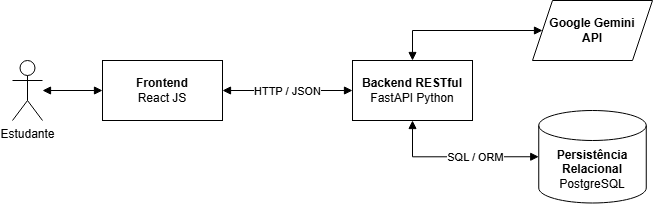
\includegraphics[width=0.9\textwidth]{figuras/arquitetura_to_be.png}
    
    \small Fonte: Elaborado pelo autor.
\end{figure}

\subsection{(A2.1) Estratégias de Inteligência Artificial e Mitigação de Limitações}

Definida a infraestrutura de base que sustentará o software, a segunda frente da Análise de Viabilidade Técnica concentrou-se na otimização do motor de Inteligência Artificial. O ambiente letivo exige o suporte a sessões síncronas com um volume simultâneo de 40 a 50 estudantes. A transição da prova de conceito para um ambiente de produção definitivo exigiu uma avaliação voltada à escolha do provedor do modelo de linguagem de grande porte (LLM), à estratégia de transmissão de dados e ao dimensionamento de contexto. A seleção estratégica do provedor da API de Inteligência Artificial, priorizando suporte de concorrência e sustentabilidade orçamentária, é fundamentada na Tabela \ref{tab:adr05}.

{
\footnotesize 
\renewcommand{\arraystretch}{1.1}

\begin{xltabular}{\textwidth}{|p{4.5cm}|X|}
    \caption{Registro de Decisão Arquitetural (ADR 05): Provedor da API de Inteligência Artificial}
    \label{tab:adr05} \\
    \toprule
    \textbf{Estrutura} & \textbf{Descrição} \\
    \midrule
    \endfirsthead

    \multicolumn{2}{c}%
    {{\bfseries \tablename\ \thetable{} -- continuação da página anterior}} \\
    \toprule
    \textbf{Estrutura} & \textbf{Descrição} \\
    \midrule
    \endhead

    \midrule \multicolumn{2}{r}{{Continua na próxima página...}} \\
    \endfoot

    \bottomrule
    \multicolumn{2}{c}{\small Fonte: Elaborada pelo autor.} \\
    \endlastfoot
    
    \textbf{Contexto e Problema} & A prova de conceito operava com envio cumulativo de histórico em camada gratuita de API, dimensionada para testes individuais, o que não suportaria rajadas de concorrência em sala de aula. É necessário definir um provedor de Modelo de Linguagem (LLM) capaz de absorver o tráfego síncrono sem bloqueios por limite de taxa (\textit{Rate Limits}), mantendo custo sustentável. \\
    \midrule
    \textbf{Opções Consideradas} & 
    \textbullet~Ecossistema Google (Gemini 3.1 Flash-Lite). \newline
    \textbullet~Ecossistema DeepSeek (DeepSeek V4 Flash). \newline
    \textbullet~Ecossistema OpenAI (GPT-5 Nano ou GPT-4o-mini). \newline
    \textbullet~Execução local descentralizada via Ollama (modelos de 5B a 8B parâmetros). \\
    \midrule
    \textbf{Opção Escolhida} & Ecossistema Google (Gemini 3.1 Flash-Lite) operando no \textit{Tier} 1 de faturamento. \\
    \midrule
    \textbf{Justificativa} & O Gemini 3.1 Flash-Lite oferece o equilíbrio ideal entre custo, continuidade da inteligência base e resiliência de infraestrutura. Modelos concorrentes da OpenAI apresentam desvantagens financeiras acentuadas: o GPT-4o-mini possui uma política de recuperação de \textit{cache} limitada a apenas 50\% de desconto, o que eleva a estimativa de gasto mensal, enquanto o GPT-5 Nano, embora econômico, exigiria a quebra de dependências e a reescrita de chamadas previamente validadas. Embora a API da DeepSeek ofereça taxas nominais agressivas, ela não publica limites rígidos e gerencia sua vazão dinamicamente com base no tráfego global, o que traria riscos de erros HTTP 503 (\textit{Server Overloaded}) em horários de pico letivo. A ativação do Gemini no \textit{Tier} 1 eleva a vazão para 300 requisições por minuto, garantindo suporte integral aos picos síncronos dos alunos com segurança orçamentária via travas de gastos (\textit{Hard Stop}). Avaliou-se também a hipótese de eliminar custos de API executando modelos locais compactos (de 5B a 8B parâmetros, como Llama 3 ou Qwen 2.5) via Ollama em contêineres Docker nas máquinas dos próprios estudantes, mas a abordagem mostrou-se inviável por três fatores: (i) degradação cognitiva em \textit{Structured Outputs}, visto que modelos de pequeno porte quantizados apresentam falhas recorrentes ao processar simultaneamente um \textit{System Prompt} denso, a memória do projeto e a geração de esquemas JSON complexos; (ii) barreira de \textit{hardware} discente, pois a ausência de GPUs dedicadas na maioria dos computadores pessoais de uma turma de 45 alunos forçaria a inferência via CPU, elevando a latência para minutos por turno; e (iii) perda de controle experimental e de telemetria centralizada em banco de dados. Optou-se, assim, por concentrar o empacotamento Docker no servidor e direcionar o esforço de pesquisa para a engenharia de \textit{prompt} e calibração de geração do modelo em nuvem (como a validação determinística de esquemas). \\
    \midrule
    \textbf{Consequências Positivas} & 
    \textbullet~Viabilidade financeira (custo mensal projetado inferior a US\$ 25) impulsionada pelo mecanismo de \textit{Context Caching}, que concede 90\% de desconto fixo para a leitura de históricos reaproveitados. \newline
    \textbullet~Compatibilidade com programas de créditos educacionais (\textit{Google Cloud Teaching Credits}) para financiamento docente integral via e-mail @unb.br. \newline
    \textbullet~Suporte a taxas de concorrência adequadas para a sala de aula. \newline
    \textbullet~Continuidade tecnológica direta com a base da prova de conceito original. \\
    \midrule
    \textbf{Consequências Negativas} & 
    \textbullet~Dependência de monitoramento constante dos ciclos de faturamento da plataforma. \newline
    \textbullet~Necessidade de acompanhamento dos cronogramas de depreciação de versões pelo provedor. \\
\end{xltabular}
}

Com o ecossistema do provedor definido, a avaliação voltou-se para a otimização da comunicação entre o \textit{backend} da aplicação e a interface da inteligência artificial, visando eliminar a redundância de tráfego herdada da prova de conceito. A Tabela \ref{tab:adr06} documenta a decisão arquitetural de unificar o processamento conversacional e a extração estruturada de requisitos em uma única chamada de API.

{
\footnotesize 
\renewcommand{\arraystretch}{1.1}

\begin{xltabular}{\textwidth}{|p{4.5cm}|X|}
    \caption{Registro de Decisão Arquitetural (ADR 06): Unificação de Chamadas da API via Saídas Estruturadas}
    \label{tab:adr06} \\
    \toprule
    \textbf{Estrutura} & \textbf{Descrição} \\
    \midrule
    \endfirsthead

    \multicolumn{2}{c}%
    {{\bfseries \tablename\ \thetable{} -- continuação da página anterior}} \\
    \toprule
    \textbf{Estrutura} & \textbf{Descrição} \\
    \midrule
    \endhead

    \midrule \multicolumn{2}{r}{{Continua na próxima página...}} \\
    \endfoot

    \bottomrule
    \multicolumn{2}{c}{\small Fonte: Elaborada pelo autor.} \\
    \endlastfoot
    
    \textbf{Contexto e Problema} & A arquitetura da prova de conceito realizava duas chamadas HTTP independentes à API do LLM por turno (uma para condução do \textit{chat} com 342 \textit{tokens} de \textit{prompt} e outra para extração com 165 \textit{tokens}). Em escala de turma, esse modelo duplica o tráfego do histórico conversacional a cada mensagem, elevando o consumo de \textit{tokens} de entrada, a latência de rede e o risco de dessincronização entre a resposta textual e o artefato extraído. \\
    \midrule
    \textbf{Opções Consideradas} & 
    \textbullet~Manter o fluxo de duas chamadas paralelas em \textit{background} (Abordagem da PoC original). \newline
    \textbullet~Unificar os \textit{prompts} em uma única chamada síncrona com retorno em formato de texto livre. \newline
    \textbullet~Unificar os \textit{prompts} em uma chamada única com Saídas Estruturadas (\textit{Structured Outputs via JSON Schema}). \\
    \midrule
    \textbf{Opção Escolhida} & Unificar os \textit{prompts} em uma chamada única com Saídas Estruturadas (\textit{Structured Outputs via JSON Schema}). \\
    \midrule
    \textbf{Justificativa} & A unificação através de saídas estruturadas nativas da API do Gemini 3.1 permite que o modelo processe o histórico de conversação apenas uma vez por turno, executando a análise semântica e a geração dialógica de forma atômica. Isso elimina a redundância de rede, reduz o consumo de \textit{tokens} de entrada em relação ao modelo duplo e garante consistência, pois a mesma instância lógica gera o diálogo e formata simultaneamente o objeto JSON contendo as histórias de usuário e critérios de aceitação. \\
    \midrule
    \textbf{Consequências Positivas} & 
    \textbullet~Redução imediata do volume bruto de entrada. \newline
    \textbullet~Maior garantia de sincronia e integridade em tempo real entre o \textit{chat} e as entidades salvas. \newline
    \textbullet~Simplificação do código no \textit{backend} (FastAPI), eliminando rotinas complexas de paralelismo síncrono. \\
    \midrule
    \textbf{Consequências Negativas} & 
    \textbullet~Pequeno acréscimo no volume de \textit{tokens} de saída devido à sintaxe rígida do formato JSON (chaves, aspas e delimitadores de propriedades). \newline
    \textbullet~Exige validação do esquema recebido no \textit{backend} antes da persistência. \\
\end{xltabular}
}

Embora a unificação das rotas reduza o desperdício estrutural, a natureza cumulativa das interações com modelos de linguagem exige o reenvio contínuo do histórico de mensagens a cada turno. Para evitar que esse acúmulo esgote os limites de banda da rede ao longo da aula, definiu-se uma estratégia de corte lógico. O estabelecimento de uma Janela Deslizante de Contexto (\textit{Sliding Window}), projetada para ancorar a quantidade de \textit{tokens} transmitidos, é apresentado na Tabela \ref{tab:adr07}.

{
\footnotesize 
\renewcommand{\arraystretch}{1.1}

\begin{xltabular}{\textwidth}{|p{4.5cm}|X|}
    \caption{Registro de Decisão Arquitetural (ADR 07): Controle e Dimensionamento de Contexto}
    \label{tab:adr07} \\
    \toprule
    \textbf{Estrutura} & \textbf{Descrição} \\
    \midrule
    \endfirsthead

    \multicolumn{2}{c}%
    {{\bfseries \tablename\ \thetable{} -- continuação da página anterior}} \\
    \toprule
    \textbf{Estrutura} & \textbf{Descrição} \\
    \midrule
    \endhead

    \midrule \multicolumn{2}{r}{{Continua na próxima página...}} \\
    \endfoot

    \bottomrule
    \multicolumn{2}{c}{\small Fonte: Elaborada pelo autor.} \\
    \endlastfoot
    
    \textbf{Contexto e Problema} & A natureza da elicitação de requisitos gera um fenômeno de ``inchaço de contexto'' (\textit{context bloat}), onde dezenas de mensagens acumuladas tornam as requisições HTTP sucessivamente mais pesadas. Além de elevar exponencialmente o consumo da API, \textit{prompts} inflados provocam atrasos de rede e lentidão no tempo de resposta para os estudantes. \\
    \midrule
    \textbf{Opções Consideradas} & 
    \textbullet~Envio integral e cumulativo do histórico (Abordagem da PoC). \newline
    \textbullet~Janela Deslizante de Contexto (\textit{Sliding Window}) simples. \newline
    \textbullet~Janela Deslizante com Fixação de Prefixo (\textit{Pinned Prompt}). \\
    \midrule
    \textbf{Opção Escolhida} & Janela Deslizante com Fixação de Prefixo (\textit{Pinned Prompt}). \\
    \midrule
    \textbf{Justificativa} & Para maximizar o desconto estrutural de 90\% na leitura de \textit{cache} oferecido nativamente pelo modelo escolhido, a arquitetura fixará o extenso \textit{System Prompt} (as regras de domínio e a persona de elicitação) como um prefixo imutável no topo de toda requisição. Simultaneamente, o histórico de interações do aluno passará por uma \textit{Sliding Window}, descartando as mensagens mais antigas e limitando o envio de dados novos apenas aos $N$ turnos mais recentes. Essa sinergia estaciona o consumo de \textit{tokens} em um teto linear e altamente previsível. \\
    \midrule
    \textbf{Consequências Positivas} & 
    \textbullet~Otimização drástica do tempo de resposta da API. \newline
    \textbullet~Proteção financeira contra progressões aritméticas de consumo. \newline
    \textbullet~Garantia de estabilidade da persona, uma vez que as diretrizes do modelo ficam ``ancoradas'' de forma permanente. \\
    \midrule
    \textbf{Consequências Negativas} & 
    \textbullet~O descarte mecânico das interações intermediárias desencadeia um quadro previsível de ``amnésia algorítmica'', fazendo o LLM esquecer restrições citadas no início da sessão. \\
\end{xltabular}
}

A implementação da Janela Deslizante (Tabela \ref{tab:adr07}) estabiliza o tamanho das requisições em um patamar de transmissão otimizado, impedindo a degradação temporal da API. Entretanto, a exclusão sistêmica de mensagens antigas causa a perda imediata de referências latentes. Um requisito funcional abordado brevemente pelo aluno nos primeiros turnos da sessão, caso não seja iterado, será descartado do horizonte de visão da IA, fragmentando o modelo de dados e invalidando a elicitação.

O impacto deste descarte torna-se sistêmico em aplicações contínuas (nas quais os alunos retomam seus projetos em aulas subsequentes), pois a limpeza de memória implícita (\textit{Time To Live}) dos servidores do provedor exige o restabelecimento do contexto de forma integral. Com o intuito de solucionar esta limitação, sem incorrer na reversão da Janela Deslizante, projetou-se uma arquitetura baseada em gerenciamento híbrido de memória no servidor, estruturada de forma complementar e detalhada na Tabela \ref{tab:adr08}.

{
\footnotesize 
\renewcommand{\arraystretch}{1.1}

\begin{xltabular}{\textwidth}{|p{4.5cm}|X|}
    \caption{Registro de Decisão Arquitetural (ADR 08): Mitigação de Perda de Contexto (Memória Híbrida)}
    \label{tab:adr08} \\
    \toprule
    \textbf{Estrutura} & \textbf{Descrição} \\
    \midrule
    \endfirsthead

    \multicolumn{2}{c}%
    {{\bfseries \tablename\ \thetable{} -- continuação da página anterior}} \\
    \toprule
    \textbf{Estrutura} & \textbf{Descrição} \\
    \midrule
    \endhead

    \midrule \multicolumn{2}{r}{{Continua na próxima página...}} \\
    \endfoot

    \bottomrule
    \multicolumn{2}{c}{\small Fonte: Elaborada pelo autor.} \\
    \endlastfoot
    
    \textbf{Contexto e Problema} & A implementação da Janela Deslizante (ADR 07) soluciona o gargalo de consumo, mas introduz um risco fatal para a Engenharia de Requisitos: a deleção de definições valiosas mencionadas no início da conversa. É imperativo adotar um sistema de memória que preserve as regras de negócio a longo prazo sem inflacionar a requisição atual. \\
    \midrule
    \textbf{Opções Consideradas} & 
    \textbullet~Memória de Resumo Contínuo (\textit{Summary Memory}). \newline
    \textbullet~Memória de Entidades Persistidas (\textit{Entity Memory} / Extração em \textit{Background}). \newline
    \textbullet~Estratégia de Memória Híbrida (Resumo + Entidades). \\
    \midrule
    \textbf{Opção Escolhida} & Estratégia de Memória Híbrida (Resumo + Entidades). \\
    \midrule
    \textbf{Justificativa} & A adoção conjunta das abordagens reduz as limitações individuais de cada uma. Ao interagir, as mensagens descartadas pela janela deslizante acionarão uma rotina enxuta de Memória de Resumo, responsável por preservar o tom e a fluidez do fluxo de diálogo. Além disso, os requisitos formalizados serão persistidos no PostgreSQL como Entidades Extraídas (reaproveitando as rotinas assíncronas já mapeadas na versão original) e injetados ativamente no \textit{prompt} estático. \\
    \midrule
    \textbf{Consequências Positivas} & 
    \textbullet~Prevenção da degradação de atenção (\textit{Lost in the Middle}) \cite{liu2023}. \newline
    \textbullet~Rastreabilidade analítica rigorosa dos requisitos no banco de dados. \newline
    \textbullet~Habilidade de o sistema retomar interações passadas em dias diferentes sem necessidade de reprocessar históricos colossais. \\
    \midrule
    \textbf{Consequências Negativas} & 
    \textbullet~Elevação substancial da complexidade de desenvolvimento no \textit{backend}, exigindo a implementação de \textit{frameworks} de orquestração (como LangChain\footnote{LangChain. Documentação Oficial. Disponível em: \url{https://docs.langchain.com/}. Acesso em: 18 jun. 2026.}) no FastAPI para gerenciar o roteamento dinâmico de resumos e extrações. \\
\end{xltabular}
}

A consolidação dessa mecânica de mitigação de custos e proteção contra a degradação de contexto é centralizada no motor de orquestração da aplicação. O fluxo lógico deste processo de montagem de \textit{payload} é detalhado na Figura \ref{fig:orquestracao_memoria}. 

\begin{figure}[H]
    \centering
    \caption{Fluxograma da Orquestração de Memória (Janela Deslizante e Memória Híbrida)}
    \label{fig:orquestracao_memoria}
    
    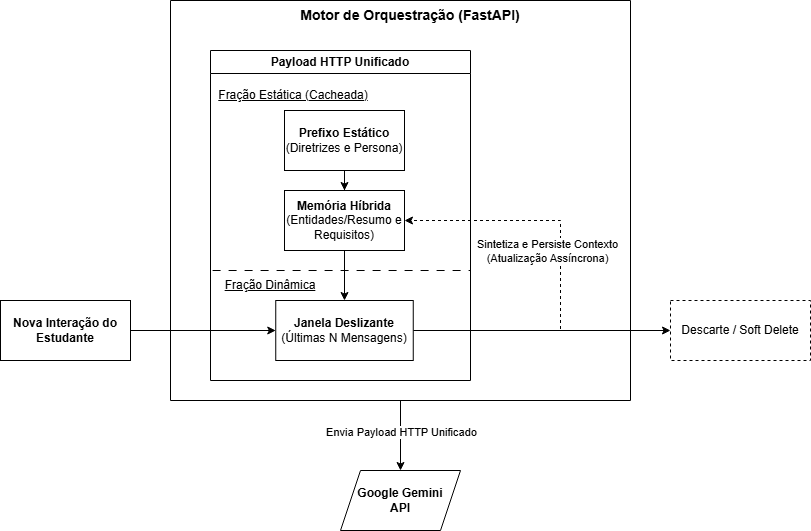
\includegraphics[width=0.9\textwidth]{figuras/orquestracao_memoria.png}
    
    \small Fonte: Elaborada pelo autor.
\end{figure}

Para validar a sustentabilidade da arquitetura proposta e mensurar o impacto conjunto das decisões documentadas nos ADRs 06, 07 e 08, modelou-se matematicamente o consumo de \textit{tokens} sob um cenário de estresse arquitetural (\textit{worst-case scenario}): duas turmas de até 50 alunos utilizando a ferramenta em todas as aulas do mês, com sessões de $n = 25$ turnos e um ``Cenário Contínuo'' longitudinal acumulando $n = 100$ turnos até a 4ª sessão. A declaração completa das variáveis extraídas do código-fonte e a memória de cálculo algébrica encontram-se disponíveis no repositório do projeto\footnote{Variáveis de arquitetura e memória de cálculo disponíveis em: \url{https://github.com/CedisUnB/ElicitBot-v2/blob/main/docs/memoria_calculo_custos.md}.}.

Aplicando a tarifação oficial do Gemini 3.1 Flash-Lite (US\$ 0,25/1M para entrada; US\$ 0,025/1M para leitura em \textit{cache}; e US\$ 1,50/1M para saída)\footnote{Preços da API Gemini 3.1 Flash-Lite. Disponível em: \url{https://ai.google.dev/gemini-api/docs/pricing?hl=pt-br\#gemini-3.1-flash-lite}. Acesso em: 18 jun. 2026.}, a Tabela \ref{tab:consumo_gemini_31} consolida a projeção comparativa de consumo e custos.

{
\footnotesize 
\renewcommand{\arraystretch}{1.1}

\begin{xltabular}{\textwidth}{|X|p{2.6cm}|p{2.6cm}|p{2.3cm}|p{1.8cm}|}
    \caption{Comparativo de Consumo e Projeção Financeira da Aplicação \\ (Gemini 3.1 Flash-Lite)}
    \label{tab:consumo_gemini_31} \\
    \toprule
    \textbf{Cenário Arquitetural} & \textbf{Volume Bruto de Entrada (Tokens/Aluno na Sessão)} & \textbf{Volume Gerado de Saída (Tokens/Aluno na Sessão)} & \textbf{Custo Estimado (Por Aluno na Sessão)} & \textbf{Projeção Mensal} \\
    \midrule
    \endfirsthead

    \multicolumn{5}{c}%
    {{\bfseries \tablename\ \thetable{} -- continuação da página anterior}} \\
    \toprule
    \textbf{Cenário Arquitetural} & \textbf{Volume Bruto de Entrada (Tokens/Aluno na Sessão)} & \textbf{Volume Gerado de Saída (Tokens/Aluno na Sessão)} & \textbf{Custo Estimado (Por Aluno na Sessão)} & \textbf{Projeção Mensal} \\
    \midrule
    \endhead

    \midrule \multicolumn{5}{r}{{Continua na próxima página...}} \\
    \endfoot

    \bottomrule
    \multicolumn{5}{c}{\small Fonte: Elaborada pelo autor.} \\
    \endlastfoot

    Linha de Base: PoC Original (Sessão Isolada de 25 turnos) & 360.175 & 13.750 & US\$ 0,110 & US\$ 95,80 \\
    \midrule
    Pós-ADR 06: Chamada Única Unificada (Sessão Isolada de 25 turnos) & 257.500 & 16.250 & US\$ 0,088 & US\$ 76,80 \\
    \midrule
    Pós-ADR 06 (Escala Contínua): Efeito Avalanche na 4ª Sessão consecutiva (Turnos 76 a 100) & 1.757.500 & 16.250 & US\$ 0,463 & US\$ 401,50 \\
    \midrule
    Pós-ADRs 07 e 08 (Arquitetura Final): Escala Contínua Imune ao Tempo (4ª Sessão e subsequentes) & 110.000 & 16.250 & US\$ 0,046 & US\$ 39,81 \\
\end{xltabular}
}

Os indicadores demonstram que, em sessões longitudinais contínuas apoiadas apenas na unificação de chamadas (ADR 06), o acúmulo linear do histórico produziria um ``Efeito Avalanche'', atingindo 1,75 milhão de \textit{tokens} de entrada por aluno na quarta sessão (US\$ 401,50 mensais). A combinação da Janela Deslizante (ADR 07) com a Memória Híbrida (ADR 08) e o desconto de 90\% do \textit{Context Caching} estabiliza o volume bruto de entrada no teto fixo de 110.000 \textit{tokens} e reduz a projeção mensal para US\$ 39,81 (aproximadamente R\$ 210,00), mitigando simultaneamente a degradação de atenção (\textit{Lost in the Middle}) \cite{liu2023}. A Figura \ref{fig:efeito_avalanche} ilustra o contraste entre as curvas de tráfego.

\begin{figure}[H]
    \centering
    \caption{Projeção de Tráfego: Efeito Avalanche vs. Escala Estabilizada}
    \label{fig:efeito_avalanche}
    
    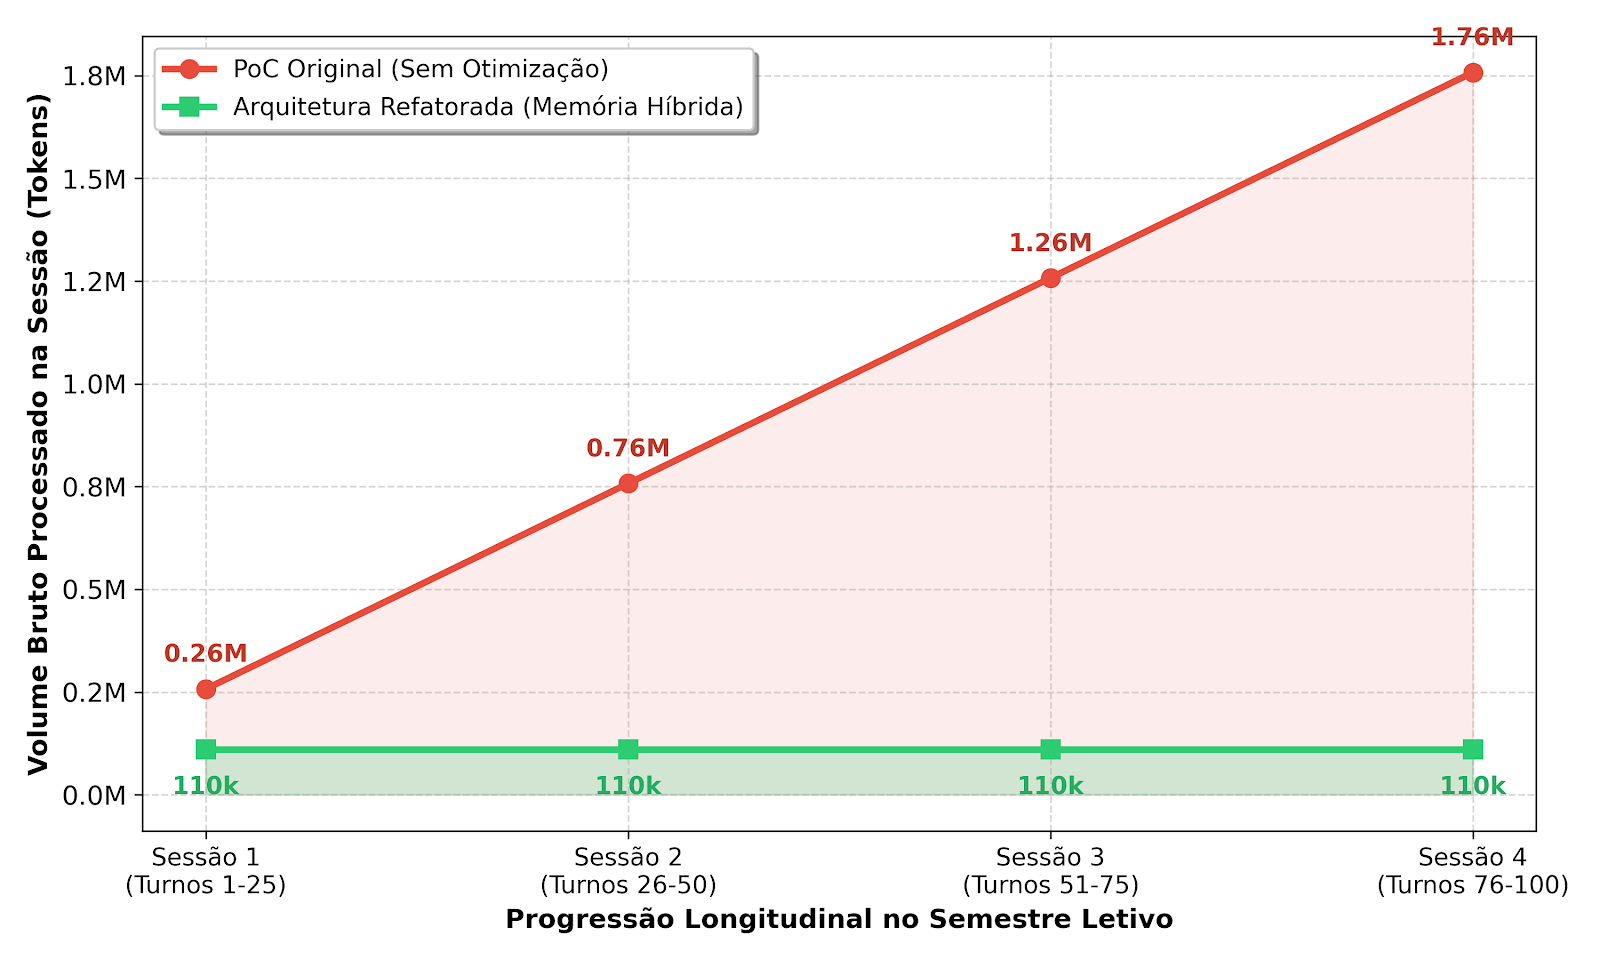
\includegraphics[width=0.9\textwidth]{figuras/efeito_avalanche.png}
    
    \small Fonte: Elaborada pelo autor a partir de \textit{script} Python gerado por IA (Gemini).
\end{figure}

Como estratégia de contingência orçamentária (\textit{Fallback Strategy}) para os ciclos de desenvolvimento e testes de carga, modelou-se também a operação sob o modelo antecedente Gemini 2.5 Flash-Lite (tarifado a US\$ 0,10/1M para entrada, US\$ 0,01/1M para leitura em \textit{cache} e US\$ 0,40/1M para saída)\footnote{Preços da API Gemini 2.5 Flash-Lite. Disponível em: \url{https://ai.google.dev/gemini-api/docs/pricing?hl=pt-br\#gemini-2.5-flash-lite}. Acesso em: 18 jun. 2026.}, conforme detalhado na Tabela \ref{tab:consumo_gemini_25}.

{
\footnotesize 
\renewcommand{\arraystretch}{1.1}

\begin{xltabular}{\textwidth}{|X|p{2.6cm}|p{2.6cm}|p{2.3cm}|p{1.8cm}|}
    \caption{Comparativo de Consumo e Projeção Financeira da Aplicação \\ (Gemini 2.5 Flash-Lite)}
    \label{tab:consumo_gemini_25} \\
    \toprule
    \textbf{Cenário Arquitetural} & \textbf{Volume Bruto de Entrada (Tokens/Aluno na Sessão)} & \textbf{Volume Gerado de Saída (Tokens/Aluno na Sessão)} & \textbf{Custo Estimado (Por Aluno na Sessão)} & \textbf{Projeção Mensal} \\
    \midrule
    \endfirsthead

    \multicolumn{5}{c}%
    {{\bfseries \tablename\ \thetable{} -- continuação da página anterior}} \\
    \toprule
    \textbf{Cenário Arquitetural} & \textbf{Volume Bruto de Entrada (Tokens/Aluno na Sessão)} & \textbf{Volume Gerado de Saída (Tokens/Aluno na Sessão)} & \textbf{Custo Estimado (Por Aluno na Sessão)} & \textbf{Projeção Mensal} \\
    \midrule
    \endhead

    \midrule \multicolumn{5}{r}{{Continua na próxima página...}} \\
    \endfoot

    \bottomrule
    \multicolumn{5}{c}{\small Fonte: Elaborada pelo autor.} \\
    \endlastfoot

    Linha de Base: PoC Original (Sessão Isolada de 25 turnos) & 360.175 & 13.750 & US\$ 0,041 & US\$ 36,00 \\
    \midrule
    Pós-ADR 06: Chamada Única Unificada (Sessão Isolada de 25 turnos) & 257.500 & 16.250 & US\$ 0,032 & US\$ 27,90 \\
    \midrule
    Pós-ADR 06 (Escala Contínua): Efeito Avalanche na 4ª Sessão da semana (Turnos 76 a 100) & 1.757.500 & 16.250 & US\$ 0,182 & US\$ 157,80 \\
    \midrule
    Pós-ADRs 07 e 08 (Arquitetura Final): Escala Contínua Imune ao Tempo (4ª Sessão e subsequentes) & 110.000 & 16.250 & US\$ 0,0151 & US\$ 13,11 \\
\end{xltabular}
}

Sob essa configuração alternativa, o custo mensal projetado reduz-se para US\$ 13,11 (aproximadamente R\$ 70,00), assegurando viabilidade financeira mesmo em cenário de autofinanciamento, com possibilidade de alternância transparente de modelo via variáveis no servidor.

\subsection{(A2.1) Estruturação do Backlog Técnico da Refatoração}

A partir da consolidação da Análise de Viabilidade Técnica e da aprovação dos oito Registros de Decisão Arquitetural (ADRs), o plano de evolução do ElicitBot foi decomposto em pacotes de trabalho acionáveis. Para guiar a fase de engenharia e garantir o alinhamento estrito entre o planejamento estratégico e a implementação prática, estruturou-se o \textit{Backlog} Técnico do projeto.

As tarefas foram distribuídas em uma matriz dimensional estruturada em três Frentes de Trabalho fundamentais (Infraestrutura Base, Orquestração de Inteligência Artificial e Interface de Usuário), acompanhadas de seus respectivos critérios de aceitação e índices de rastreabilidade arquitetural, conforme consolidado na Tabela \ref{tab:backlog_tecnico}.

\noindent
{
\footnotesize 
\renewcommand{\arraystretch}{1.1}
\setlength{\LTleft}{0pt}
\setlength{\LTright}{0pt}

\begin{xltabular}{\textwidth}{|p{1.8cm}|p{3.2cm}|X|X|p{1.7cm}|}
    \caption{Backlog Técnico Inicial para a Refatoração do Sistema}
    \label{tab:backlog_tecnico} \\
    \toprule
    \textbf{Frente / ID} & \textbf{Nome da Tarefa} & \textbf{Descrição Técnica} & \textbf{Critérios de Aceitação} & \textbf{Rastreab.} \\
    \midrule
    \endfirsthead

    \multicolumn{5}{c}%
    {{\bfseries \tablename\ \thetable{} -- continuação da página anterior}} \\
    \toprule
    \textbf{Frente / ID} & \textbf{Nome da Tarefa} & \textbf{Descrição Técnica} & \textbf{Critérios de Aceitação} & \textbf{Rastreab.} \\
    \midrule
    \endhead

    \midrule \multicolumn{5}{r}{{Continua na próxima página...}} \\
    \endfoot

    \bottomrule
    \multicolumn{5}{c}{\small Fonte: Elaborada pelo autor.} \\
    \endlastfoot
    
    \textbf{Frente 1} & \multicolumn{4}{p{\dimexpr\textwidth-2.5cm\relax}|}{\textbf{Infraestrutura Base:} Configuração do ecossistema de desenvolvimento e isolamento de camadas do servidor.} \\
    \midrule
    T1.01 & Inicialização do \textit{Backend} em FastAPI & Configurar o ambiente virtual Python, instalar dependências do \textit{framework} FastAPI e estruturar a árvore de diretórios (rotas, controladores e esquemas). & 
    \textbullet~Servidor inicializando localmente. \newline
    \textbullet~Rota de \textit{health-check} operacional. \newline
    \textbullet~Swagger UI gerada. & 
    ADR 02 \\
    \midrule
    T1.02 & Modelagem e Provisionamento do PostgreSQL & Estabelecer a \textit{string} de conexão com a instância relacional e mapear os modelos ORM para a persistência estruturada de Projetos, Sessões, Mensagens e Requisitos. & 
    \textbullet~Conexão validada via \textit{logs}. \newline
    \textbullet~Tabelas geradas via \textit{migration}. \newline
    \textbullet~Chaves estrangeiras funcionais. \newline
    \textbullet~\textit{Soft Delete} (\texttt{is\_ativo}) operante. \newline
    \textbullet~Operações de CRUD executadas com sucesso. & 
    ADR 03 \\
    \midrule
    T1.03 & Preparação do Ambiente de \textit{Deploy} & Estruturar os manifestos de empacotamento com o Docker\footnote{Docker. Documentação Oficial. Disponível em: \url{https://docs.docker.com/}. Acesso em: 18 jun. 2026.} e \textit{scripts} de inicialização compatíveis com a infraestrutura institucional. & 
    \textbullet~Aplicação encapsulada no ambiente. \newline
    \textbullet~Inicialização via linha de comando simulada. & 
    ADR 04 \\
    \midrule
    T1.04 & Implementação de Observabilidade (\textit{Logs}) & Configurar um \textit{logger} estruturado no FastAPI para capturar exceções, requisições HTTP e latência das chamadas de IA. & 
    \textbullet~\textit{Logs} formatados com \textit{timestamp}/nível. \newline
    \textbullet~Registro de falhas/erros com a API do Gemini. & 
    ADR 02 / 05 \\
    \midrule
    T1.05 & Controle de Acesso e \textit{Rate Limiting} & Implementar autenticação via Microsoft Entra ID e construir interceptadores no FastAPI para bloqueio de janela letiva e \textit{throttling}. & 
    \textbullet~Login restrito a e-mails institucionais cadastrados. \newline
    \textbullet~\textit{Middleware} retorna HTTP 403 fora do horário para funções de conversa com o agente. \newline
    \textbullet~\textit{Middleware} retorna HTTP 429 se exceder o limite de chamadas. & 
    ADR 02 \\
    \midrule
    T1.06 & Implementação de \textit{Schemas} e Repositórios (CRUD) & Implementar a camada de isolamento do banco de dados (padrão \textit{Repository}) e os contratos de validação de dados da API (\textit{Schemas} Pydantic\footnote{Pydantic. Documentação Oficial. Disponível em: \url{https://pydantic.dev/docs/}. Acesso em: 18 jun. 2026.}) para todas as entidades persistidas. & 
    \textbullet~Modelos mapeados possuem \textit{Schemas} de entrada (\textit{Create}/\textit{Update}) e saída (\textit{Response}). \newline
    \textbullet~Classes de Repositório implementadas para encapsular operações CRUD do SQLAlchemy. \newline
    \textbullet~Exceções de tabelas associativas puras documentadas. & 
    ADR 02 / 03 \\
    \midrule
    \textbf{Frente 2} & \multicolumn{4}{p{\dimexpr\textwidth-2.5cm\relax}|}{\textbf{Orquestração de IA e Memória:} Implementação lógica do motor cognitivo e gerenciamento de eficiência de \textit{tokens}.} \\
    \midrule
    T2.01 & Integração Unificada com LLM via Saídas Estruturadas & Acoplar o SDK do Gemini 3.1 Flash-Lite no FastAPI e unificar os \textit{prompts} forçando o retorno nativo em formato JSON Schema. & 
    \textbullet~API realiza chamada única por turno. \newline
    \textbullet~Retorno atômico de texto e matriz JSON. \newline
    \textbullet~Erros sintáticos mitigados pelo Pydantic. & 
    ADR 05 / 06 \\
    \midrule
    T2.02 & Algoritmo de Janela Deslizante (\textit{Sliding Window}) & Desenvolver o interceptador de estado para fixar o \textit{prompt} do sistema no prefixo e rotacionar o histórico bruto de mensagens. & 
    \textbullet~Carga limitada aos últimos $N$ turnos. \newline
    \textbullet~\textit{System Prompt} imutável no topo do pacote. & 
    ADR 07 \\
    \midrule
    T2.03 & Mecanismo de Memória Híbrida & Construir rotinas assíncronas em \textit{background} para atualizar o resumo e reinjetar as entidades extraídas do PostgreSQL. & 
    \textbullet~A IA mantém ciência de requisitos antigos. \newline
    \textbullet~Resumos gerados dentro do teto de 500 \textit{tokens}. & 
    ADR 08 \\
    \midrule
    T2.04 & Otimização de Custos (\textit{Context Caching}) & Configurar a API do Gemini para registrar formalmente o Prefixo Estático como um \textit{CachedContent}. & 
    \textbullet~Tarifa de \textit{cache} aplicada na fração estática. \newline
    \textbullet~Renovação do \textit{cache} apenas na alteração do banco ou após $N$ turnos conversacionais. & 
    ADR 07 / 08 \\
    \midrule
    \textbf{Frente 3} & \multicolumn{4}{p{\dimexpr\textwidth-2.5cm\relax}|}{\textbf{Interface de Elicitação:} Reconstrução da camada visual e consumo assíncrono das rotas estruturadas.} \\
    \midrule
    T3.01 & Construção do Ambiente React & Inicializar o ecossistema \textit{frontend} em React, padronizando componentes globais de interface e rotas de navegação. & 
    \textbullet~Interface responsiva livre de \textit{warnings}. \newline
    \textbullet~Telas de \textit{Dashboard} e \textit{chat} acessíveis. \newline
    \textbullet~Mecanismos de controle (\textit{Undo}, edição) visíveis. & 
    ADR 01 \\
    \midrule
    T3.02 & Integração e Renderização Síncrona & Conectar componentes do React aos \textit{endpoints} do FastAPI, dividindo a tela entre o fluxo de diálogo e a tabela de requisitos. & 
    \textbullet~Envio de mensagens sem travamento da tela. \newline
    \textbullet~Atualização reativa imediata da listagem lateral. & 
    ADR 01 / 06 \\
\end{xltabular}
}

A conclusão deste \textit{Backlog} Técnico encerra o planejamento da arquitetura interna e as atividades de validação de infraestrutura da fase A2.1. O sistema encontra-se mapeado do ponto de vista do desenvolvedor, permitindo que a pesquisa avance para a atividade subsequente, focada em estruturar as necessidades do usuário sob a ótica de produto.

\subsection{(A2.2) Especificação e Priorização do \textit{Backlog} de Evolução Funcional}

Enquanto a atividade anterior (A2.1) solucionou a viabilidade técnica e a infraestrutura interna do sistema, a atividade A2.2 concentrou-se na perspectiva de valor entregue ao usuário final. A transição de um protótipo acadêmico para uma ferramenta de produção exigiu o mapeamento claro de como as interações lógicas apoiariam o estudante e o docente no laboratório de Engenharia de Requisitos.

Para cumprir esse objetivo, estruturou-se o \textit{Backlog} Funcional inicial do sistema por meio de Histórias de Usuário (\textit{User Stories}), adotando dois perfis de atores: \textbf{estudante} (usuário final que conduz a elicitação) e \textbf{administrador} (docente ou pesquisador responsável pela governança da plataforma, cujo perfil herda hierarquicamente todas as permissões de acesso e autenticação do estudante). Essa modelagem garantiu a paridade funcional (\textit{feature parity}) com os requisitos essenciais validados na Prova de Conceito original (Requisitos R1 a R6 da Tabela \ref{tab:requisitos_originais}), expandindo-os com capacidades de gerenciamento de projetos, controle de acesso institucional e edição humana (\textit{Human-in-the-Loop}).

Visando orientar o fluxo de desenvolvimento e delimitar o Subconjunto Mínimo Utilizável (\textit{Minimum Usable Subset}) do Produto Mínimo Viável (MVP), o escopo foi priorizado utilizando a matriz técnica MoSCoW \cite{agilebusiness2014}:

\begin{itemize}
    \item \textbf{\textit{Must Have} (Deve ter):} Funcionalidades vitais sem as quais o sistema perde seu propósito principal ou torna-se inseguro para operação em sala de aula (autenticação, criação e recuperação de projetos, ativação de travas de acesso e horário, condução conversacional, extração e exportação).
    \item \textbf{\textit{Should Have} (Deveria ter):} Funcionalidades de alto valor agregado, incluindo operações de manutenção do ciclo de vida de registros (edição de títulos, limpeza de testes e revogação de regras) e mecanismos de controle \textit{Human-in-the-Loop}, mas cuja ausência temporária não inviabilizaria a execução básica da sessão.
    \item \textbf{\textit{Could Have} (Poderia ter):} Requisitos desejáveis de transparência e \textit{feedback} granular em nível de \textit{card}, implementados caso haja viabilidade de tempo no cronograma.
    \item \textbf{\textit{Won't Have} (Não terá desta vez):} Funcionalidades complexas fora do escopo atual, documentadas para compor os trabalhos futuros.
\end{itemize}

As 23 funcionalidades planejadas inicialmente foram agrupadas em três Épicos fundamentais, detalhados e priorizados na Tabela \ref{tab:backlog_funcional}.

\noindent
{
\footnotesize 
\renewcommand{\arraystretch}{1.15}
\setlength{\LTleft}{0pt}
\setlength{\LTright}{0pt}

\begin{xltabular}{\textwidth}{|l|>{\raggedright\arraybackslash}p{4.0cm}|>{\raggedright\arraybackslash}X|p{1.9cm}|>{\raggedright\arraybackslash}p{2.2cm}|}
    \caption{Backlog Funcional Inicial do Sistema\protect\footnotemark}
    \label{tab:backlog_funcional} \\
    \toprule
    \textbf{ID} & \textbf{História de Usuário} & \textbf{Critérios de Aceitação (Síntese)} & \textbf{Prioridade} & \textbf{Origem / Requisito} \\
    \midrule
    \endfirsthead

    \multicolumn{5}{c}%
    {{\bfseries \tablename\ \thetable{} -- continuação da página anterior}} \\
    \toprule
    \textbf{ID} & \textbf{História de Usuário} & \textbf{Critérios de Aceitação (Síntese)} & \textbf{Prioridade} & \textbf{Origem / Requisito} \\
    \midrule
    \endhead

    \midrule \multicolumn{5}{r}{{Continua na próxima página...}} \\
    \endfoot

    \bottomrule
    \multicolumn{5}{c}{\small Fonte: Elaborada pelo autor.} \\
    \endlastfoot
    
    \textbf{Épico 1} & \multicolumn{4}{p{\dimexpr\textwidth-2.2cm\relax}|}{\textbf{Controle de Acesso e Gestão de Projetos}} \\
    \midrule
    US1.01 & Como estudante, quero iniciar um novo projeto, para organizar uma nova sessão de elicitação isolada. & 
    Modal exige nome obrigatório (bloqueando envio vazio); \texttt{POST /api/projetos} persiste o registro, inicializa estado na fase \texttt{contexto} com mensagem de boas-vindas e redireciona ao \textit{workspace} (\texttt{201 Created}). & 
    \textit{Must Have} & Trabalhos Futuros (PoC) \\
    \midrule
    US1.02 & Como estudante, quero visualizar todos os meus projetos em formato de \textit{cards} no painel principal, para localizar e acessar sessões anteriores rapidamente. & 
    \texttt{GET /api/projetos} lista projetos ordenados por \texttt{updated\_at DESC}; renderização em \textit{cards} com data formatada, indicador de carregamento (\textit{spinner}) e tratamento de \textit{empty state}. & 
    \textit{Must Have} & Trabalhos Futuros (PoC) \\
    \midrule
    US1.03 & Como estudante, quero editar o título de um projeto já criado, para corrigir erros de digitação. & 
    \texttt{PATCH /api/projetos/\{id\}} valida propriedade (\texttt{403 Forbidden} se inválido); modal preenchido com nome atual, validação contra vazio e atualização instantânea na tela. & 
    \textit{Should Have} & Trabalhos Futuros (PoC) \\
    \midrule
    US1.04 & Como estudante, quero excluir projetos criados para testes ou desnecessários, para manter minha área de trabalho limpa e organizada. & 
    \texttt{DELETE /api/projetos/\{id\}} valida autoria (\texttt{403}/\texttt{404}) e aplica \textit{soft delete} sem deixar órfãos; exige modal de confirmação prévio e remove o \textit{card} de forma fluida (\texttt{204}). & 
    \textit{Should Have} & Trabalhos Futuros (PoC) \\
    \midrule
    US1.05 & Como estudante, quero acessar o histórico de um projeto existente, para continuar a elicitação de onde parei. & 
    Rotas \texttt{/mensagens} e \texttt{/artefatos} validam acesso (\texttt{403}/\texttt{404}); carrega histórico cronológico do \textit{chat}, preenche a barra lateral com os artefatos salvos e bloqueia IDs inválidos. & 
    \textit{Must Have} & Trabalhos Futuros (PoC) \\
    \midrule
    US1.06 & Como administrador, quero cadastrar e-mails autorizados, para que apenas alunos matriculados tenham acesso ao ElicitBot. & 
    Validação contra campo vazio; \texttt{POST /emails} bloqueia duplicatas (\texttt{400 Bad Request}), converte para caixa baixa e atualiza dinamicamente a lista (\texttt{201 Created}). & 
    \textit{Must Have} & Novo (Segurança / \textit{FinOps}) \\
    \midrule
    US1.07 & Como administrador, quero visualizar a lista de e-mails autorizados, para auditar quem tem acesso ao sistema no momento. & 
    \texttt{GET /emails} retorna todos os e-mails autorizados em \textit{card} de \textit{Whitelist}, exibindo mensagem de \textit{empty state} caso a base esteja vazia. & 
    \textit{Must Have} & Novo (Segurança / \textit{FinOps}) \\
    \midrule
    US1.08 & Como administrador, quero remover e-mails da \textit{whitelist}, para revogar o acesso de alunos após o término da disciplina. & 
    Exclusão via \texttt{DELETE /emails/\{id\}} com modal de confirmação (\texttt{204}); oculta botão e bloqueia no \textit{backend} (\texttt{400}) a exclusão de contas de administradores. & 
    \textit{Should Have} & Novo (Segurança / \textit{FinOps}) \\
    \midrule
    US1.09 & Como administrador, quero definir janelas de horário e dias da semana, para restringir as respostas do LLM aos momentos da disciplina. & 
    Valida início $<$ término; \texttt{POST /horarios} cadastra regra e dependência bloqueia rotas de IA (\texttt{POST /mensagens} e \texttt{DELETE /ultimo-turno}) fora da janela (\texttt{403}), mantendo leitura e exportação livres. & 
    \textit{Must Have} & Novo (Segurança / \textit{FinOps}) \\
    \midrule
    US1.10 & Como administrador, quero visualizar todas as janelas letivas configuradas, para consultar os horários ativos da ferramenta. & 
    \texttt{GET /horarios} lista horários ativos com dia traduzido e hora formatada (\texttt{HH:MM}), exibindo alerta de bloqueio 24/7 caso não existam regras. & 
    \textit{Must Have} & Novo (Segurança / \textit{FinOps}) \\
    \midrule
    US1.11 & Como administrador, quero excluir janelas letivas previamente configuradas, para desativar o sistema em férias ou feriados. & 
    Exclusão via \texttt{DELETE /horarios/\{id\}} após confirmação (\texttt{204}), interrompendo imediatamente novas interações com o LLM caso a janela estivesse vigente. & 
    \textit{Should Have} & Novo (Segurança / \textit{FinOps}) \\
    \midrule
    US1.12 & Como estudante, quero me autenticar utilizando minha conta institucional via Microsoft ID (SSO), para acessar sem criar novas senhas. & 
    Fluxo OAuth2/OIDC via botão ``Entrar com Microsoft'', emissão de JWT interno após validar \textit{whitelist}, redirecionamento ao \textit{Dashboard} e alerta amigável se não autorizado. & 
    \textit{Must Have} & Novo (Segurança / \textit{FinOps}) \\
    \midrule
    US1.13 & Como estudante, quero encerrar minha sessão ativamente (\textit{Logout}), para garantir a privacidade em computadores compartilhados. & 
    Botão ``Sair'' remove o JWT local, aciona \textit{logout} no provedor Microsoft, invalida o estado global de autenticação e bloqueia retorno às rotas protegidas. & 
    \textit{Must Have} & Novo (Segurança / \textit{FinOps}) \\
    \midrule
    \textbf{Épico 2} & \multicolumn{4}{p{\dimexpr\textwidth-2.2cm\relax}|}{\textbf{Motor de Elicitação Inteligente}} \\
    \midrule
    US2.01 & Como estudante, quero dialogar em linguagem natural com o assistente, para ser guiado ativamente na elicitação de requisitos. & 
    Condução investigativa com espelhamento, detecção de ambiguidades/conflitos e sugestão de encerramento; indicador ``Analisando...'' e bloqueio do \textit{input} durante resposta da IA. & 
    \textit{Must Have} & Req. 1, 2 e 3 (PoC) / Trab. Futuros \\
    \midrule
    US2.02 & Como estudante, quero visualizar histórias de usuário em formato padrão e compreensível, para validar se minhas necessidades foram capturadas. & 
    Atualização síncrona da barra lateral a cada turno extraído, obedecendo estritamente ao padrão ``Como [papel], quero [ação] para [benefício]''. & 
    \textit{Must Have} & Req. 4 e 5 (PoC) \\
    \midrule
    US2.03 & Como estudante, quero editar manualmente as histórias de usuário geradas, para corrigir interpretações equivocadas da IA. & 
    Botão de edição abre modal preenchido com os dados atuais do artefato, permitindo edições parciais que atualizam o banco e a memória do LLM. & 
    \textit{Should Have} & Trabalhos Futuros (PoC) \\
    \midrule
    US2.04 & Como estudante, quero excluir o meu último turno de conversa, para corrigir falhas de raciocínio enviadas por engano. & 
    Botão ``Desfazer'' (desabilitado sem histórico ou durante requisição) que remove atomicamente o turno e aplica \textit{soft delete} em cascata nos artefatos gerados nele. & 
    \textit{Should Have} & Trabalhos Futuros (PoC) \\
    \midrule
    US2.05 & Como estudante, quero visualizar a justificativa metodológica por trás das perguntas do assistente, para compreender as técnicas aplicadas. & 
    Campo opcional \texttt{justificativa\_metodologica} no JSON da IA renderizado em componente expansível (``Modo Pensamento'') abaixo da mensagem no \textit{chat}. & 
    \textit{Could Have} & Novo (Transparência Pedagógica) \\
    \midrule
    US2.06 & Como estudante, quero que o assistente também identifique e estruture Requisitos Não Funcionais (RNFs), para abranger necessidades arquiteturais. & 
    Extração declarativa verificável categorizada (FURPS+ / ISO 25010), com aba exclusiva na barra lateral, edição manual e seção dedicada na exportação. & 
    \textit{Won't Have} & Novo (Expansão Técnica) \\
    \midrule
    US2.07 & Como estudante, quero enviar mensagens de voz (\textit{speech-to-text}), para tornar a elicitação semelhante a uma entrevista presencial. & 
    Gravação via microfone no navegador com transcrição via API externa inserida na caixa de texto para revisão manual antes do envio. & 
    \textit{Won't Have} & Req. 7 (PoC) / Trab. Futuros \\
    \midrule
    \textbf{Épico 3} & \multicolumn{4}{p{\dimexpr\textwidth-2.2cm\relax}|}{\textbf{Consumação e Avaliação}} \\
    \midrule
    US3.01 & Como estudante, quero exportar o \textit{Backlog} consolidado em múltiplos formatos (PDF, Markdown e JSON), para anexá-lo à documentação acadêmica. & 
    Exportação de todos os artefatos e \textit{Tags} de rastreabilidade no padrão \texttt{[Projeto]\_DRS.[ext]}, omitindo metadados internos no JSON e tratando ausência de RFs com aviso amigável. & 
    \textit{Must Have} & Req. 6 (PoC) / Trab. Futuros \\
    \midrule
    US3.02 & Como estudante, quero avaliar individualmente a utilidade dos requisitos gerados, para apontar quais captações foram mais precisas. & 
    Ícones positivo/negativo exclusivos nos \textit{cards} de Requisitos Funcionais, exibindo campo de texto opcional para justificativa em caso de avaliação negativa. & 
    \textit{Could Have} & Req. 9 (PoC) / Novo (Métricas) \\
    \midrule
    US3.03 & Como estudante, quero exportar as histórias de usuário diretamente para serviços como Jira/Trello/GitHub Projects, para automatizar a gestão. & 
    Conexão OAuth2 com plataforma externa, seleção de quadro, mapeamento automático em \textit{issues/cards} com relatório de \textit{links} e tratamento de falhas (\textit{retries}). & 
    \textit{Won't Have} & Trabalhos Futuros (PoC) \\
\end{xltabular}
}
\footnotetext{A especificação integral dos critérios de aceitação de todas as Histórias de Usuário encontra-se disponível no repositório do projeto em: \url{https://github.com/CedisUnB/ElicitBot-v2/blob/main/docs/backlog_funcional.md}.}

A estruturação deste \textit{Backlog} Funcional inicial, priorizado pela técnica MoSCoW, foi alinhada e validada junto ao \textit{stakeholder} do projeto (professor orientador), estabelecendo uma distribuição equilibrada em conformidade com as boas práticas do \textit{framework} DSDM \cite{agilebusiness2014}:

\begin{itemize}
    \item \textbf{\textit{Must Have} (Deve ter, 12 histórias ou 52,2\%):} Requisitos vitais correspondentes à paridade funcional da Prova de Conceito (PoC) original (US2.01, US2.02 e US3.01), à criação, listagem e recuperação persistente de projetos (US1.01, US1.02 e US1.05) e à ativação dos controles de segurança, autenticação institucional e trava de horário letivo (US1.06, US1.07, US1.09, US1.10, US1.12 e US1.13).
    \item \textbf{\textit{Should Have} (Deveria ter, 6 histórias ou 26,1\%):} Funcionalidades importantes de manutenção e organização do ciclo de vida dos registros (edição de título e exclusão de projetos em US1.03 e US1.04; revogação de e-mails e de janelas letivas em US1.08 e US1.11) e mecanismos essenciais de controle e correção pelo usuário (\textit{Human-in-the-Loop}: edição manual em US2.03 e reversão de turno em US2.04).
    \item \textbf{\textit{Could Have} (Poderia ter, 2 histórias ou 8,7\%):} Funcionalidades desejáveis de apoio pedagógico e coleta complementar, abrangendo a exibição da justificativa metodológica por pergunta (US2.05) e a avaliação individual de utilidade nos \textit{cards} de requisitos (US3.02), condicionadas à disponibilidade de cronograma após a entrega das prioridades superiores.
    \item \textbf{\textit{Won't Have} (Não terá desta vez, 3 histórias ou 13,0\%):} Funcionalidades fora do escopo desta pesquisa, como estruturação de Requisitos Não Funcionais (US2.06), envio de mensagens por voz \textit{speech-to-text} (US2.07) e integração via API com plataformas externas como Jira, Trello e GitHub Projects (US3.03), documentadas exclusivamente para compor os trabalhos futuros.
\end{itemize}

Com isso, encerrou-se formalmente a Fase 1 de diagnóstico e planejamento do projeto. Com as dimensões de infraestrutura, limites operacionais de \textit{tokens}, persistência de estado e necessidades iniciais de produto especificadas, os documentos produzidos serviram como diretriz operacional para a execução da Fase 2 de refatoração e desenvolvimento, detalhada na seção a seguir.

\section{Fase 2: Refatoração e Desenvolvimento}
\label{sec:execucao_fase2}

Concluído o planejamento arquitetural e a priorização inicial de escopo na Fase 1, a pesquisa avançou para a execução do Ciclo de Design da DSR, compreendendo a refatoração estrutural do sistema (A3.1), o desenvolvimento incremental das funcionalidades de produto (A3.2) e a validação de estabilidade sob carga (A3.3).

\subsection{(A3.1) Implementação do plano de ação para resolver os problemas de escalabilidade}
\label{subsec:exec_a31}

A execução da atividade A3.1 iniciou-se pela implementação das tarefas de infraestrutura e desacoplamento previstas no \textit{Backlog} Técnico inicial (Tabela \ref{tab:backlog_tecnico}).

\subsubsection*{Infraestrutura Base, Persistência Transacional e Ambiente de \textit{Deploy} (T1.01 a T1.06)}

Seguindo as diretrizes dos ADRs 01, 02 e 03, a aplicação foi reestruturada em uma arquitetura cliente-servidor desacoplada. O \textit{backend} foi construído em Python com o \textit{framework} assíncrono FastAPI (\textbf{T1.01}), organizado segundo os padrões de Arquitetura em Camadas (\textit{Layered Architecture}), \textit{Repository} e \textit{Service Layer}, com validação estrita de contratos de entrada e saída via esquemas Pydantic (\textbf{T1.06}). A camada de persistência foi implementada no banco de dados relacional PostgreSQL 16 (\textbf{T1.02}) por meio do mapeamento objeto-relacional (ORM) assíncrono SQLAlchemy 2.0 e controle de migrações via Alembic, segmentando o ciclo de vida dos registros conforme a finalidade de cada entidade:

\begin{itemize}
    \item \textbf{Entidades de escopo e conversação (\texttt{Projeto}, \texttt{Mensagem} e artefatos):} operam sob exclusão lógica (\textit{soft delete}, via atributo \texttt{is\_ativo}) e bloqueio transacional pessimista na geração de identificadores sequenciais, suportando a reversão segura de turnos (\textit{undo});
    \item \textbf{Entidade de controle de acesso (\texttt{EmailAutorizado}):} opera sob exclusão física (\textit{hard delete}), atuando como condição binária de autorização na lista de permissões (\textit{whitelist});
    \item \textbf{Entidades de telemetria e avaliação (\texttt{MetricaLLM} e \texttt{AvaliacaoRequisitoFuncional}):} modeladas como registros imutáveis (\textit{append-only}), sendo que a entidade de avaliação preserva uma cópia estática (\textit{snapshot}) do requisito no instante do registro para assegurar a integridade dos dados empíricos.
\end{itemize}

Para evitar o esgotamento do \textit{pool} de conexões do banco de dados (\textit{Connection Starvation}) durante as chamadas à API do LLM, que demandam de 3 a 18 segundos de espera de rede, foi implementado o padrão transacional \textbf{\textit{Read-Release-Write}} dividido em três etapas. Primeiramente, o \textit{backend} abre uma sessão rápida para leitura do contexto do projeto e registro do horário de envio, executando o \texttt{commit} imediato para devolver a conexão ao \textit{pool}. Em seguida, realiza a chamada externa ao modelo de linguagem sem reter recursos do PostgreSQL. Por fim, ao receber a resposta validada, abre uma nova transação rápida exclusivamente para persistir de forma atômica as mensagens do turno, as operações sobre artefatos e os dados de telemetria.

Na camada de governança e observabilidade (\textbf{T1.04} e \textbf{T1.05}), foi estruturada uma pilha de interceptadores (\textit{middlewares}) na borda da API. O primeiro módulo (\texttt{LogRequestsMiddleware}) foi integrado à biblioteca \textit{Loguru} para serializar eventos, latências e pilhas de erro (\textit{tracebacks}) em formato JSON, contando com rotação automática de 10 MB e retenção de 15 dias. O segundo módulo (\texttt{ThrottlingMiddleware}) aplica uma janela deslizante de 60 segundos em memória que limita cada usuário a 100 requisições por minuto nas rotas gerais e a 10 requisições por minuto na rota de acionamento da IA, retornando o código \texttt{HTTP 429} em caso de excesso. Nas rotas de negócio, a autenticação via Microsoft Entra ID (OAuth2/OIDC com emissão de JWT interno) foi associada a verificações de dependência que validam a presença do estudante na \textit{whitelist} e bloqueiam o acionamento do LLM fora das janelas letivas (\texttt{HTTP 403}).

Para a implantação em produção (\textbf{T1.03}, ADR 04), o sistema foi conteinerizado por meio das ferramentas \textit{Docker} e \textit{Docker Compose}, isolando o servidor de aplicação (FastAPI/Uvicorn), o servidor web e \textit{proxy} reverso (Nginx) e o banco de dados (PostgreSQL), sendo disponibilizado sob subdomínio institucional do grupo de pesquisa com criptografia HTTPS (SSL/TLS).
% O servidor institucional contou com a seguinte configuração: \textbf{[TODO: Inserir especificações do servidor institucional -- Processador/vCPUs, RAM, Armazenamento e SO]}.

\subsubsection*{Evolução do Motor Conversacional e do \textit{System Prompt} (T2.01 a T2.10 e T1.07)}

A implementação inicial do motor cognitivo (\textbf{T2.01} a \textbf{T2.04}) estabeleceu a \textbf{Arquitetura de Extração Direta (\texttt{v0.x})}, unificando a condução do diálogo e a extração de dados em uma chamada única ao modelo \textit{Gemini 3.1 Flash-Lite}. Os testes práticos dessa versão demandaram oito iterações sucessivas do \textit{System Prompt} (\texttt{v0.1} a \texttt{v0.8}) e a criação da tarefa emergente \textbf{T2.05} (atualização idempotente via \textit{Upsert} por correspondência de título) para estabilizar a decodificação da estrutura JSON e evitar a duplicação de requisitos refinados ao longo da conversa.

Ao submeter a versão \texttt{v0.8} à validação de domínio junto ao professor orientador, constatou-se que o fluxo conversacional ainda mantinha uma premissa estrutural da prova de conceito original: iniciar a interação solicitando diretamente requisitos funcionais, sem antes compreender e modelar o problema e o domínio do projeto. Para alinhar a ferramenta ao fluxo metodológico de uma entrevista real de elicitação, o motor foi reestruturado para a \textbf{Arquitetura Orientada a Estados (\texttt{v1.0})}, consolidada no \textit{prompt} \texttt{v1.0-orquestracao}. A Tabela \ref{tab:evolucao_prompts} sintetiza a evolução das versões do \textit{System Prompt}, cujos textos integrais encontram-se disponíveis no repositório oficial do projeto\footnote{Histórico completo das versões do \textit{System Prompt} disponível em: \url{https://github.com/CedisUnB/ElicitBot-v2/blob/main/docs/evolucao_system_prompts.md}.}.

\noindent
{
\footnotesize 
\renewcommand{\arraystretch}{1.1}
\setlength{\LTleft}{0pt}
\setlength{\LTright}{0pt}

\begin{xltabular}{\textwidth}{|p{2.3cm}|p{4.2cm}|X|}
    \caption{Síntese Evolutiva das Versões do \textit{System Prompt} (\texttt{v0.1} a \texttt{v1.0})}
    \label{tab:evolucao_prompts} \\
    \toprule
    \textbf{Versão} & \textbf{Comportamento Observado} & \textbf{Intervenção Arquitetural e Semântica} \\
    \midrule
    \endfirsthead

    \multicolumn{3}{c}%
    {{\bfseries \tablename\ \thetable{} -- continuação da página anterior}} \\
    \toprule
    \textbf{Versão} & \textbf{Comportamento Observado} & \textbf{Intervenção Arquitetural e Semântica} \\
    \midrule
    \endhead

    \midrule \multicolumn{3}{r}{{Continua na próxima página...}} \\
    \endfoot

    \bottomrule
    \multicolumn{3}{c}{\small Fonte: Elaborada pelo autor.} \\
    \endlastfoot
    
    \texttt{v0.1} a \texttt{v0.4} \newline (Extração Direta) & Desvio de atenção (\textit{Attention Drift}) na decodificação de listas complexas, fatiando atributos de um mesmo requisito em múltiplos objetos JSON. & Fusão dos \textit{prompts} de diálogo e extração, substituição de termos genéricos por instruções de campo, aplicação de \textit{Few-Shot Prompting} e definição de molde JSON literal. \\
    \midrule
    \texttt{v0.5} a \texttt{v0.7} \newline (Extração Direta) & Extração ansiosa (\textit{Eager Extraction}) no início da conversa e aglutinação de múltiplos atores em uma mesma História de Usuário. & Permissão explícita para retorno de lista vazia em turnos exploratórios, trava de ator e ação únicos (granularidade ágil) e regra de ``Extração Exaustiva'' agrupada por \textit{Feature}. \\
    \midrule
    \texttt{v0.8} \newline (Extração Direta) & Reescrita sutil de títulos pelo LLM durante o refinamento de regras, quebrando a verificação de \textit{Upsert} por título (\textbf{T2.05}) e duplicando \textit{cards}. & Inclusão da trava de ``Manutenção de Identidade'', proibindo alterações lexicais em títulos de requisitos já constantes na memória ativa do projeto. \\
    \midrule
    \texttt{v1.0-orquestracao} \newline (Orientada a Estados) & Início direto pela extração de funcionalidades na \texttt{v0.x}, sem modelagem prévia de contexto, problemas, partes interessadas e restrições. & Reestruturação completa para uma Máquina de Estados de 12 fases, controle de ciclo de vida de 8 artefatos via Motor de Operações por \textit{Tags} imutáveis, distinções semânticas de domínio e molde \textit{Context-Grounded Few-Shot}. \\
\end{xltabular}
}

A transição para a Arquitetura Orientada a Estados (\texttt{v1.0}) deu origem às tarefas técnicas emergentes \textbf{T2.06} a \textbf{T2.10}, além da previsão preventiva de indexação em \textbf{T1.07}. Nessa modelagem, o processo conversacional foi estruturado em uma Máquina de Estados finita de 12 etapas, conforme ilustrado na Figura \ref{fig:fluxo_elicitacao}.

\begin{figure}[H]
    \centering
    \caption{Fluxo de Elicitação em 12 Etapas da Máquina de Estados do ElicitBot}
    \label{fig:fluxo_elicitacao}
    
    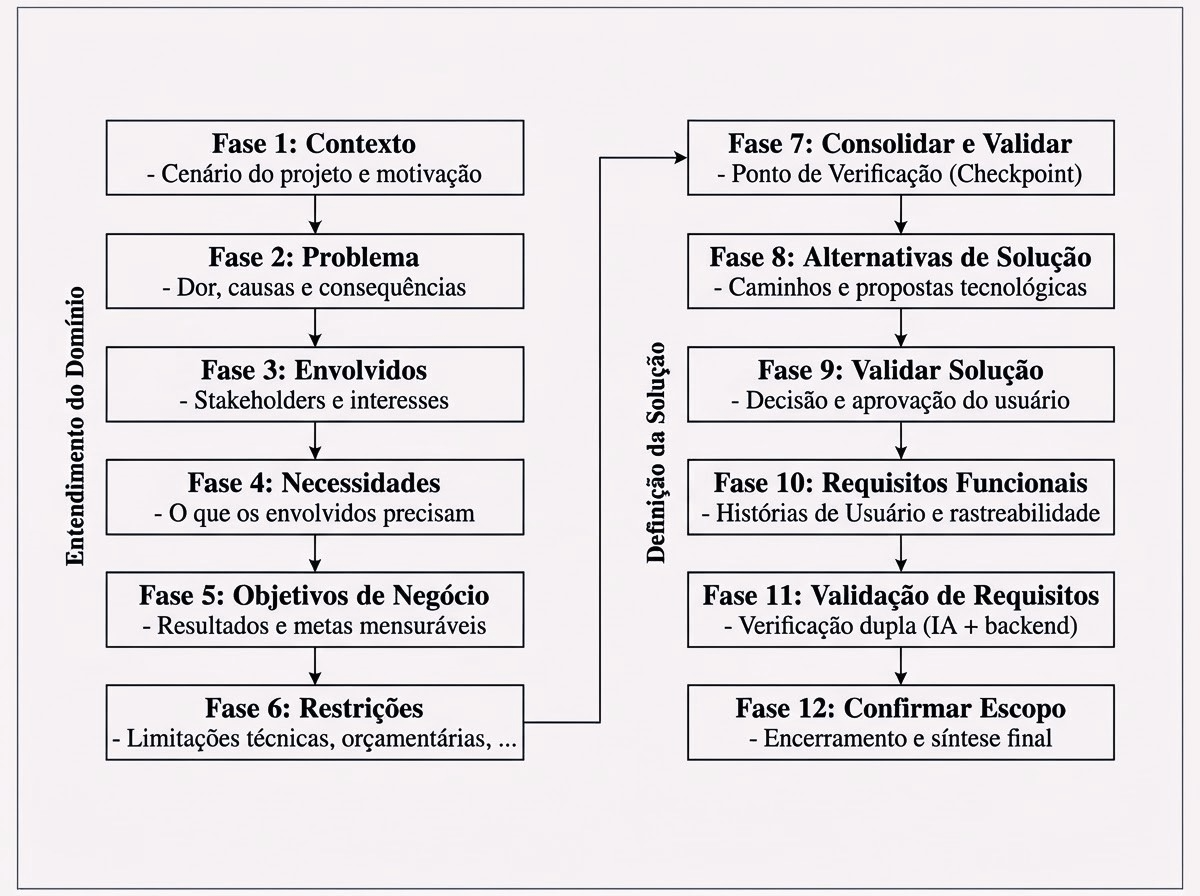
\includegraphics[width=0.92\textwidth]{figuras/fluxo_elicitacao.png}
    
    \small Fonte: Elaborada pelo autor.
\end{figure}

Para sustentar o fluxo representado na Figura \ref{fig:fluxo_elicitacao}, a arquitetura \texttt{v1.0} incorporou quatro mecanismos integrados no \textit{backend}:

\begin{enumerate}
    \item \textbf{Controle de Transição e Defesa de Escopo (T2.06):} Persistido na entidade \texttt{EstadoInteracao}, o fluxo aplica a regra de \textit{Trava de Confirmação (Gatekeeper)}, que bloqueia o avanço de fase enquanto existirem artefatos pendentes de aceite pelo usuário (\texttt{aguardando\_confirmacao}). Adicionalmente, opera a regra de \textit{Defesa do Escopo}, que armazena pedidos prematuros de funcionalidades na fila \texttt{topicos\_em\_espera} e reconduz o diálogo à fase atual, bem como o suporte à \textit{Manutenção Retroativa}, permitindo atualizar ou descartar artefatos de etapas passadas sem retroceder o ponteiro da fase vigente.
    \item \textbf{Gerenciamento Bipartido de Memória (T2.07):} O módulo construtor de contexto substituiu a sumarização textual (T2.03) pela divisão determinística do estado do banco de dados. A \textbf{Memória Estável} reúne o \textit{System Prompt} e os artefatos já \texttt{confirmados} de fases estabilizadas, sendo registrada no \textit{Context Caching} da Vertex AI com desconto de 90\% e invalidação controlada por \textit{hash} SHA-256. Por sua vez, a \textbf{Memória Dinâmica} envia fora do \textit{cache} os artefatos da fase em foco, as lacunas abertas e a janela deslizante das últimas 20 mensagens (10 turnos).
    \item \textbf{Motor de Operações e Ciclo de Vida de Artefatos (T2.08):} O Motor de Operações substituiu a rotina de \textit{Upsert} por título (T2.05) por cinco comandos explícitos (\texttt{criar}, \texttt{atualizar}, \texttt{confirmar}, \texttt{validar} e \texttt{descartar}) aplicados sobre oito tipos de artefatos identificados por \textit{Tags} sequenciais imutáveis (\texttt{CTX}, \texttt{PROB}, \texttt{ENV}, \texttt{NEC}, \texttt{OBJ}, \texttt{RES}, \texttt{SOL} e \texttt{RF}), gerenciando a transição entre os estados \texttt{aguardando\_confirmacao}, \texttt{confirmado} e \texttt{descartado}.
    \item \textbf{Dupla Validação de Requisitos Funcionais (T2.09):} Na Fase 11, os Requisitos Funcionais possuem um ciclo de validação adicional (\texttt{status\_validacao}: \texttt{nao\_validado} $\rightarrow$ \texttt{aprovado\_pelo\_backend} $\rightarrow$ \texttt{aprovado} ou \texttt{com\_pendencias}). O módulo de validação determinística do servidor audita a integridade dos vínculos, a existência de origem mínima, a cobertura de necessidades e a ausência de duplicidades lexicais antes de liberar o requisito para a validação semântica da IA.
\end{enumerate}

A Tabela \ref{tab:backlog_tecnico_emergente} consolida os sete requisitos técnicos emergentes mapeados na Fase 2.

\noindent
{
\footnotesize 
\renewcommand{\arraystretch}{1.1}
\setlength{\LTleft}{0pt}
\setlength{\LTright}{0pt}

\begin{xltabular}{\textwidth}{|p{1.4cm}|p{3.0cm}|X|X|p{2.3cm}|}
    \caption{Backlog Técnico Emergente Mapeado Durante o Desenvolvimento (Fase 2)}
    \label{tab:backlog_tecnico_emergente} \\
    \toprule
    \textbf{ID} & \textbf{Nome da Tarefa} & \textbf{Descrição Técnica} & \textbf{Critérios de Aceitação} & \textbf{Situação Final} \\
    \midrule
    \endfirsthead

    \multicolumn{5}{c}%
    {{\bfseries \tablename\ \thetable{} -- continuação da página anterior}} \\
    \toprule
    \textbf{ID} & \textbf{Nome da Tarefa} & \textbf{Descrição Técnica} & \textbf{Critérios de Aceitação} & \textbf{Situação Final} \\
    \midrule
    \endhead

    \midrule \multicolumn{5}{r}{{Continua na próxima página...}} \\
    \endfoot

    \bottomrule
    \multicolumn{5}{c}{\small Fonte: Elaborada pelo autor.} \\
    \endlastfoot
    
    T1.07 & Otimização de Consultas com Índices no Banco de Dados & Identificar padrões de consulta frequentes e implementar índices simples e compostos via migrações do Alembic para otimizar leituras e ordenações. & 
    \textbullet~Índices aplicados em chaves estrangeiras e colunas relevantes. \newline
    \textbullet~Índices compostos criados para listagem ordenada. \newline
    \textbullet~\textit{Script} de migração Alembic versionado. & 
    Não implementada (desnecessária após testes de carga) \\
    \midrule
    T2.05 & Evolução Iterativa de Requisitos (\textit{Upsert}) e Recuperação Dinâmica & Implementar mecanismo de idempotência por título para evitar duplicação de requisitos refinados ao longo de vários turnos e resgatar o JSON de requisitos antigos no \textit{prompt}. & 
    \textbullet~Busca \textit{case-insensitive} por título antes da persistência. \newline
    \textbullet~Execução de \texttt{UPDATE} em vez de \texttt{INSERT} duplicado. \newline
    \textbullet~Reatrelamento ao \texttt{mensagem\_id} atual para sincronia com o \textit{Undo}. & 
    Implementada na \texttt{v0.x} (substituída por T2.08 na \texttt{v1.0}) \\
    \midrule
    T2.06 & Implementação da Máquina de Estados de Elicitação & Substituir o fluxo de conversa livre por uma Máquina de Estados finita de 12 fases (\texttt{contexto} a \texttt{confirmacao\_escopo}), permitindo manutenção retroativa de artefatos sem retrocesso de fase. & 
    \textbullet~Instanciação automática de \texttt{EstadoInteracao} na criação do projeto. \newline
    \textbullet~Retorno de fase atual, foco, lacunas e próxima ação no JSON da IA. \newline
    \textbullet~Suporte a edição retroativa sem retorno de fase. & 
    Implementada na \texttt{v1.0} \\
    \midrule
    T2.07 & Gerenciamento Bipartido de Memória (Estável e Dinâmica) & Substituir a sumarização em \textit{background} (T2.03) por um construtor de contexto (\texttt{prompt\_builder}) que divide os artefatos do banco conforme o grau de estabilidade. & 
    \textbullet~\textit{Memória Estável}: artefatos \texttt{confirmados} de fases anteriores injetados no \textit{Context Caching}. \newline
    \textbullet~\textit{Memória Dinâmica}: artefatos da fase atual ou pendentes fora do \textit{cache}. \newline
    \textbullet~Composição unificada enviada a cada turno sem duplicação. & 
    Implementada na \texttt{v1.0} (substituiu T2.03) \\
    \midrule
    T2.08 & Motor de Operações e Ciclo de Vida dos Artefatos & Substituir o \textit{Upsert} por título (T2.05) por um Motor de Operações baseado em \textit{Tags} imutáveis, orquestrando 8 tipos de artefatos por meio de 5 comandos explícitos (\texttt{criar}, \texttt{atualizar}, \texttt{confirmar}, \texttt{validar} e \texttt{descartar}). & 
    \textbullet~Mapeamento e execução transacional das 5 operações via SQLAlchemy. \newline
    \textbullet~Tratamento isolado de validação de esquemas via Pydantic. \newline
    \textbullet~Resolução nativa de relacionamentos cruzados via \textit{Tags}. & 
    Implementada na \texttt{v1.0} (substituiu T2.05) \\
    \midrule
    T2.09 & Pré-Validação Determinística de Requisitos Funcionais & Implementar camada de verificação determinística no \textit{backend} (Fase 11) para auditar integridade de vínculos, origens mínimas e duplicidades antes da validação semântica da IA. & 
    \textbullet~Bloqueio de validação de RFs com vínculos inválidos ou não confirmados. \newline
    \textbullet~Registro automático de \texttt{pendencias\_validacao} no RF. \newline
    \textbullet~Interação guiada pela IA para sanar falhas de rastreabilidade. & 
    Implementada na \texttt{v1.0} \\
    \midrule
    T2.10 & Adequação do \textit{System Prompt} à Arquitetura Orientada a Estados & Consolidar o \textit{System Prompt} (\texttt{v1.0-orquestracao}) como contrato comportamental estrito alinhado às 12 fases da Máquina de Estados e às 5 ações do Motor de Operações. & 
    \textbullet~Descrição explícita das 12 fases e dos 8 artefatos. \newline
    \textbullet~Exigência de \textit{Tags} imutáveis como identificadores. \newline
    \textbullet~Regras de manutenção retroativa e proibição de inferências não validadas. & 
    Implementada na \texttt{v1.0} \\
\end{xltabular}
}

\subsection{(A3.2) Desenvolvimento das melhorias funcionais priorizadas}
\label{subsec:exec_a32}

Paralelamente à evolução do \textit{backend}, a atividade A3.2 executou o desenvolvimento da interface de usuário em React (utilizando TypeScript e Tailwind CSS) e das rotas previstas no \textit{Backlog} Funcional inicial (Tabela \ref{tab:backlog_funcional}). Foram implementadas integralmente todas as 18 Histórias de Usuário classificadas como \textit{Must Have} e \textit{Should Have} (\textbf{US1.01} a \textbf{US1.13}, \textbf{US2.01} a \textbf{US2.04} e \textbf{US3.01}), além da funcionalidade \textit{Could Have} voltada à avaliação individual de utilidade de Requisitos Funcionais (\textbf{US3.02}). As três histórias classificadas como \textit{Won't Have} (\textbf{US2.06}, \textbf{US2.07} e \textbf{US3.03}) permaneceram fora do escopo conforme planejado, enquanto o esforço da história \textit{Could Have} \textbf{US2.05} foi realocado para priorizar a entrega de sete Histórias de Usuário emergentes (Tabela \ref{tab:backlog_funcional_emergente}), essenciais para disponibilizar na interface a Máquina de Estados de 12 etapas, a visualização dos oito tipos de artefatos e os recursos de governança e observabilidade.

\noindent
{
\footnotesize 
\renewcommand{\arraystretch}{1.15}
\setlength{\LTleft}{0pt}
\setlength{\LTright}{0pt}

\begin{xltabular}{\textwidth}{|l|>{\raggedright\arraybackslash}p{4.0cm}|>{\raggedright\arraybackslash}X|p{1.9cm}|>{\raggedright\arraybackslash}p{2.2cm}|}
    \caption{Backlog Funcional Emergente Mapeado e Implementado na Fase 2}
    \label{tab:backlog_funcional_emergente} \\
    \toprule
    \textbf{ID} & \textbf{História de Usuário} & \textbf{Critérios de Aceitação (Síntese)} & \textbf{Prioridade} & \textbf{Origem / Motivação} \\
    \midrule
    \endfirsthead

    \multicolumn{5}{c}%
    {{\bfseries \tablename\ \thetable{} -- continuação da página anterior}} \\
    \toprule
    \textbf{ID} & \textbf{História de Usuário} & \textbf{Critérios de Aceitação (Síntese)} & \textbf{Prioridade} & \textbf{Origem / Motivação} \\
    \midrule
    \endhead

    \midrule \multicolumn{5}{r}{{Continua na próxima página...}} \\
    \endfoot

    \bottomrule
    \multicolumn{5}{c}{\small Fonte: Elaborada pelo autor.} \\
    \endlastfoot
    
    \textbf{Épico 2} & \multicolumn{4}{p{\dimexpr\textwidth-2.2cm\relax}|}{\textbf{Motor de Elicitação Inteligente (Arquitetura Orientada a Estados (\texttt{v1.0}) e Governança de Prompts)}} \\
    \midrule
    US2.08 & Como administrador, quero visualizar o histórico de versões do \textit{System Prompt}, para auditar as diretrizes da IA e identificar a versão ativa. & 
    Rota \texttt{GET /admin/prompts/} protegida por RBAC (\texttt{403}); lista expansível (\textit{accordion}) exibindo \texttt{tag\_versao}, data/hora e destaque visual para a versão ativa (\texttt{is\_ativo == True}). & 
    \textit{Could Have} & Emergente (Calibração \texttt{v1.0} / T2.10) \\
    \midrule
    US2.09 & Como administrador, quero cadastrar uma nova versão do \textit{System Prompt} pela interface, para refinar as instruções sem realizar novos \textit{deploys}. & 
    Modal pré-carrega o \textit{prompt} ativo como base; \texttt{POST /admin/prompts/} valida unicidade de \texttt{tag\_versao} (\texttt{400}), salva registro imutável e permite ativação imediata via \textit{checkbox}. & 
    \textit{Could Have} & Emergente (Calibração \texttt{v1.0} / T2.10) \\
    \midrule
    US2.10 & Como administrador, quero definir qual versão histórica do \textit{System Prompt} será a ativa, para controlar as configurações dos novos projetos. & 
    \texttt{PATCH /admin/prompts/\{id\}/ativar} alterna \texttt{is\_ativo} atomicamente após confirmação, afetando apenas novos projetos e preservando \texttt{versao\_prompt\_id} dos existentes. & 
    \textit{Could Have} & Emergente (Calibração \texttt{v1.0} / T2.10) \\
    \midrule
    US2.11 & Como estudante, quero que a entrevista seja dividida em etapas lógicas e progressivas, para não definir todo o sistema de uma só vez. & 
    Indicador visual da fase atual no painel; perguntas focadas na etapa vigente, manutenção retroativa sem retorno de fase e retenção de tópicos adiantados em espera. & 
    \textit{Must Have} & Emergente (Máquina de Estados / T2.06) \\
    \midrule
    US2.12 & Como estudante, quero visualizar todos os artefatos levantados pelo assistente (contexto, problemas, envolvidos, etc.), para validar o alinhamento. & 
    Navegação categorizada na barra lateral entre as oito tipologias de artefatos da arquitetura \texttt{v1.0}, com \textit{layout} e metadados específicos de domínio. & 
    \textit{Must Have} & Emergente (Motor de Operações / T2.08) \\
    \midrule
    \textbf{Épico 3} & \multicolumn{4}{p{\dimexpr\textwidth-2.2cm\relax}|}{\textbf{Consumação, Avaliação e Observabilidade Científica}} \\
    \midrule
    US3.04 & Como administrador, quero exportar os dados de telemetria em CSV pela interface \textit{web}, para analisar o desempenho da IA sem acesso ao banco. & 
    Restrito a \texttt{admin}; gera CSV em memória transmitido via \textit{stream} sem gravar em disco, com \textit{spinner}, bloqueio contra cliques múltiplos e tratamento de falhas. & 
    \textit{Should Have} & Emergente (Coleta Científica / ADR 04) \\
    \midrule
    US3.05 & Como administrador, quero visualizar as últimas linhas do \textit{log} no painel de controle, para diagnosticar falhas ou \textit{timeouts} sem acesso SSH. & 
    Restrito a \texttt{admin}; exibe últimas 500 linhas JSON coloridas por severidade com \textit{auto-scroll}, filtro de alertas, modal de \textit{Traceback} e \textit{download} do arquivo \texttt{.log} bruto. & 
    \textit{Should Have} & Emergente (Monitoramento / ADR 04) \\
\end{xltabular}
}

A Figura \ref{fig:tela_chat} apresenta a área de trabalho em painel duplo resultante da integração entre as histórias iniciais (\textbf{US2.01}, \textbf{US2.02}, \textbf{US2.04} e \textbf{US3.01}) e emergentes (\textbf{US2.11} e \textbf{US2.12}). À esquerda, a barra lateral reativa indica a etapa vigente da Máquina de Estados (\texttt{Envolvidos}), agrupa em abas expansíveis as oito categorias de artefatos com seus respectivos contadores e disponibiliza o botão ``Exportar Escopo'' para geração do Documento de Requisitos de Software (DRS) nos formatos PDF, Markdown e JSON. À direita, o painel conversacional conduz a entrevista, demonstrando na prática a manutenção retroativa de artefatos de fases anteriores (\texttt{PROB-02} e \texttt{Contexto}) simultaneamente à transição para a fase de \texttt{Envolvidos}, além de disponibilizar o controle de reversão de turno (``Desfazer'').

\begin{figure}[H]
    \centering
    \caption{Interface da Área de Trabalho em Painel Duplo (\textit{Chat} e Barra Lateral de Artefatos)}
    \label{fig:tela_chat}
    
    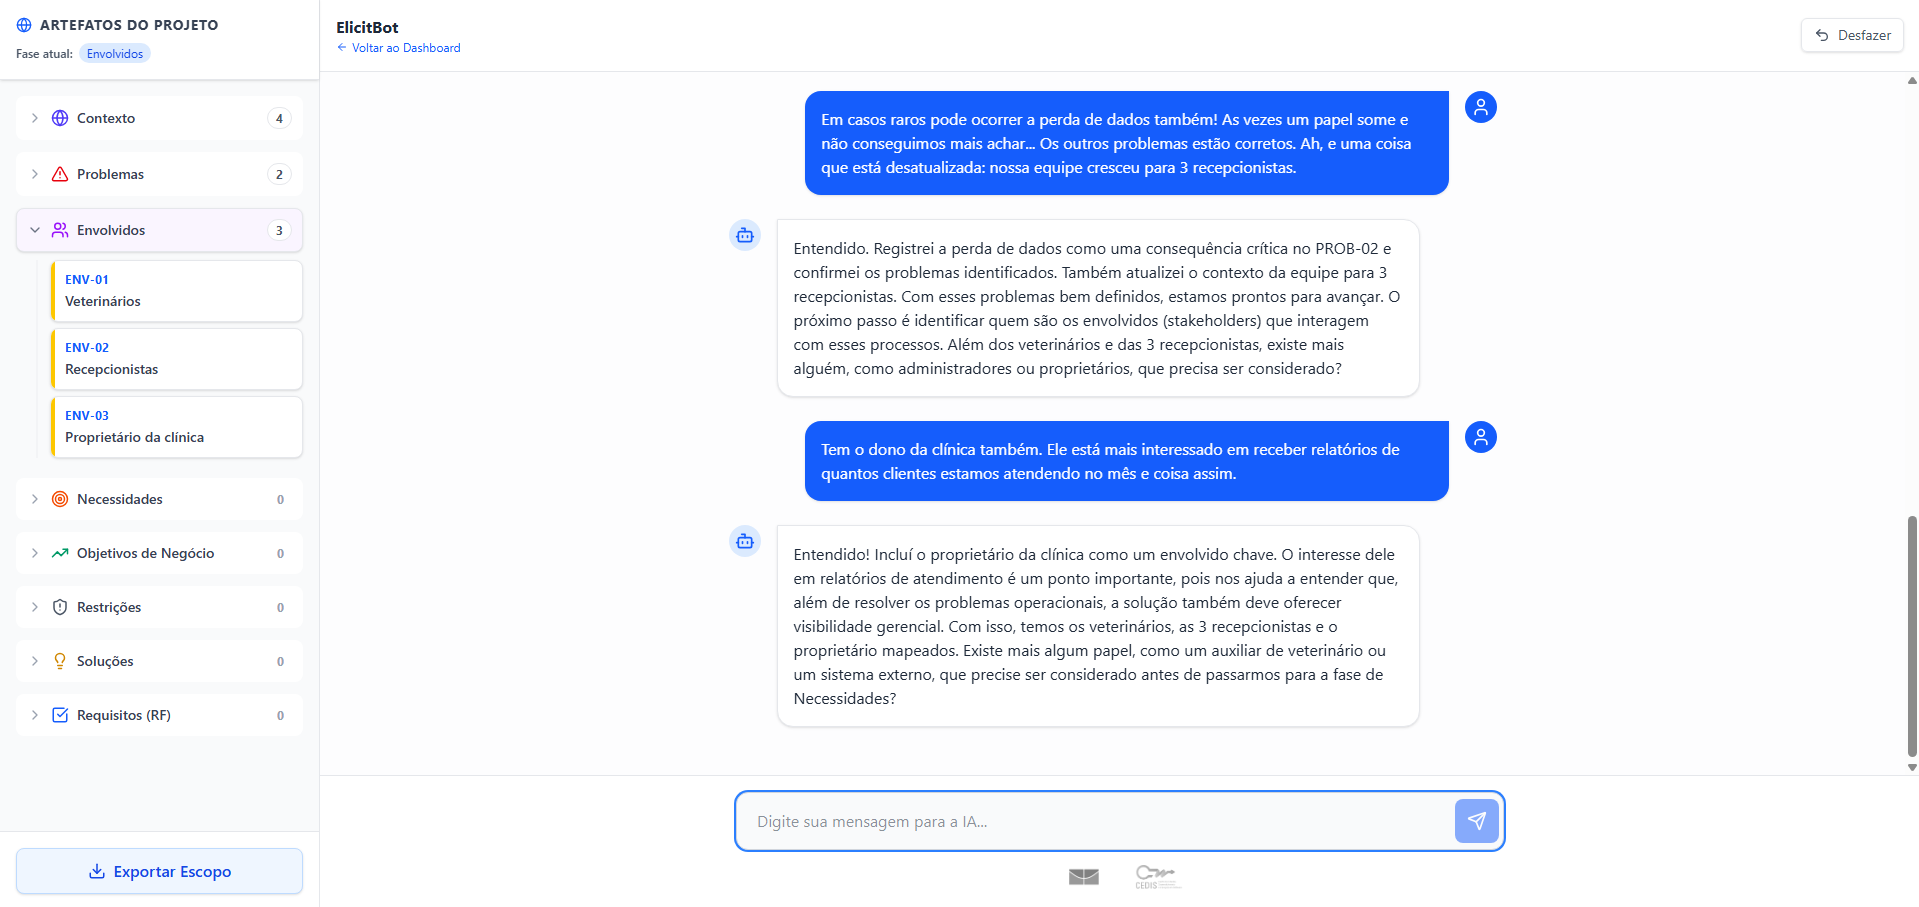
\includegraphics[width=0.96\textwidth]{figuras/tela_chat.png}
    
    \small Fonte: Elaborada pelo autor.
\end{figure}

Complementando a experiência do estudante, a Figura \ref{fig:telas_dashboard_modal} apresenta, em (a), o painel principal (\textit{Dashboard}) de gerenciamento de sessões (\textbf{US1.01} a \textbf{US1.05}) e, em (b), o modal de inspeção detalhada de artefato, acionado ao selecionar um item da barra lateral (ilustrado pelo artefato \texttt{PROB-02}). Esse componente materializa o controle \textit{Human-in-the-Loop} (\textbf{US2.03}) ao permitir a visualização estruturada e a edição manual de qualquer atributo, bem como a avaliação individual de utilidade quando aplicado a Requisitos Funcionais (\textbf{US3.02}).

\begin{figure}[H]
    \centering
    \caption{Painel Principal de Projetos (\textit{Dashboard}) e Modal de Detalhamento e Edição de Artefato}
    \label{fig:telas_dashboard_modal}
    \begin{minipage}[b]{0.48\textwidth}
        \centering
        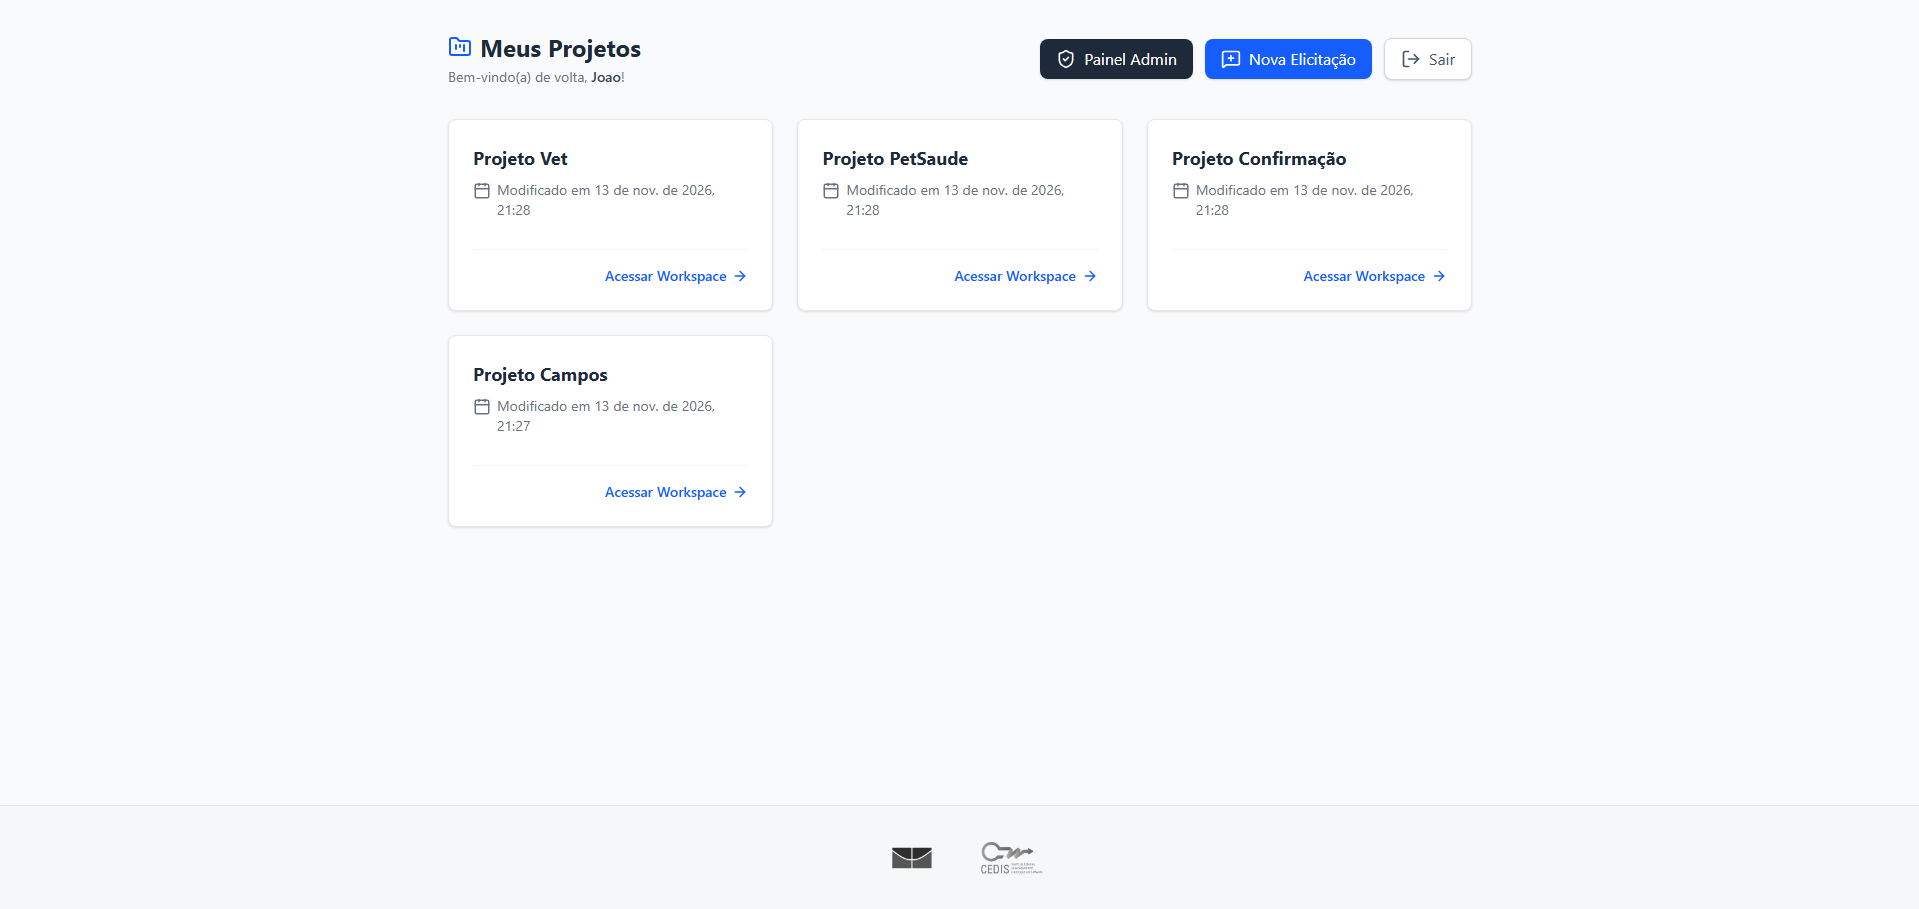
\includegraphics[trim={300px 0px 300px 0px}, clip, width=\textwidth]{figuras/tela_dashboard.png}
        \par\smallskip{\footnotesize (a) \textit{Dashboard} de gestão de projetos}
    \end{minipage}
    \hfill
    \begin{minipage}[b]{0.48\textwidth}
        \centering
        
\includegraphics[trim={420px 0px 420px 0px}, clip, width=\textwidth]{figuras/tela_modal_artefato.png}
        \par\smallskip{\footnotesize (b) Modal de detalhes e edição (\texttt{PROB-02})}
    \end{minipage}
    \par\medskip
    \small Fonte: Elaborada pelo autor.
\end{figure}

Por fim, a Figura \ref{fig:tela_admin} ilustra o Painel de Administração dividido em suas duas seções operacionais: em (a), os módulos de gerenciamento da \textit{Whitelist} de e-mails e das janelas de horário letivo (\textbf{US1.06} a \textbf{US1.11}), o botão de exportação de telemetria em CSV (\textbf{US3.04}) e o painel de governança e ativação dinâmica de versões do \textit{System Prompt} (\textit{LLMOps}, \textbf{US2.08} a \textbf{US2.10}); e, em (b), o Console do Servidor para monitoramento em tempo real das últimas 500 linhas de \textit{log}, filtro de alertas e inspeção de exceções sem necessidade de acesso SSH (\textbf{US3.05}).

\begin{figure}[H]
    \centering
    \caption{Interface do Painel de Administração: Governança de Acesso, \textit{LLMOps} e Console do Servidor}
    \label{fig:tela_admin}
    \begin{minipage}[b]{0.48\textwidth}
        \centering
        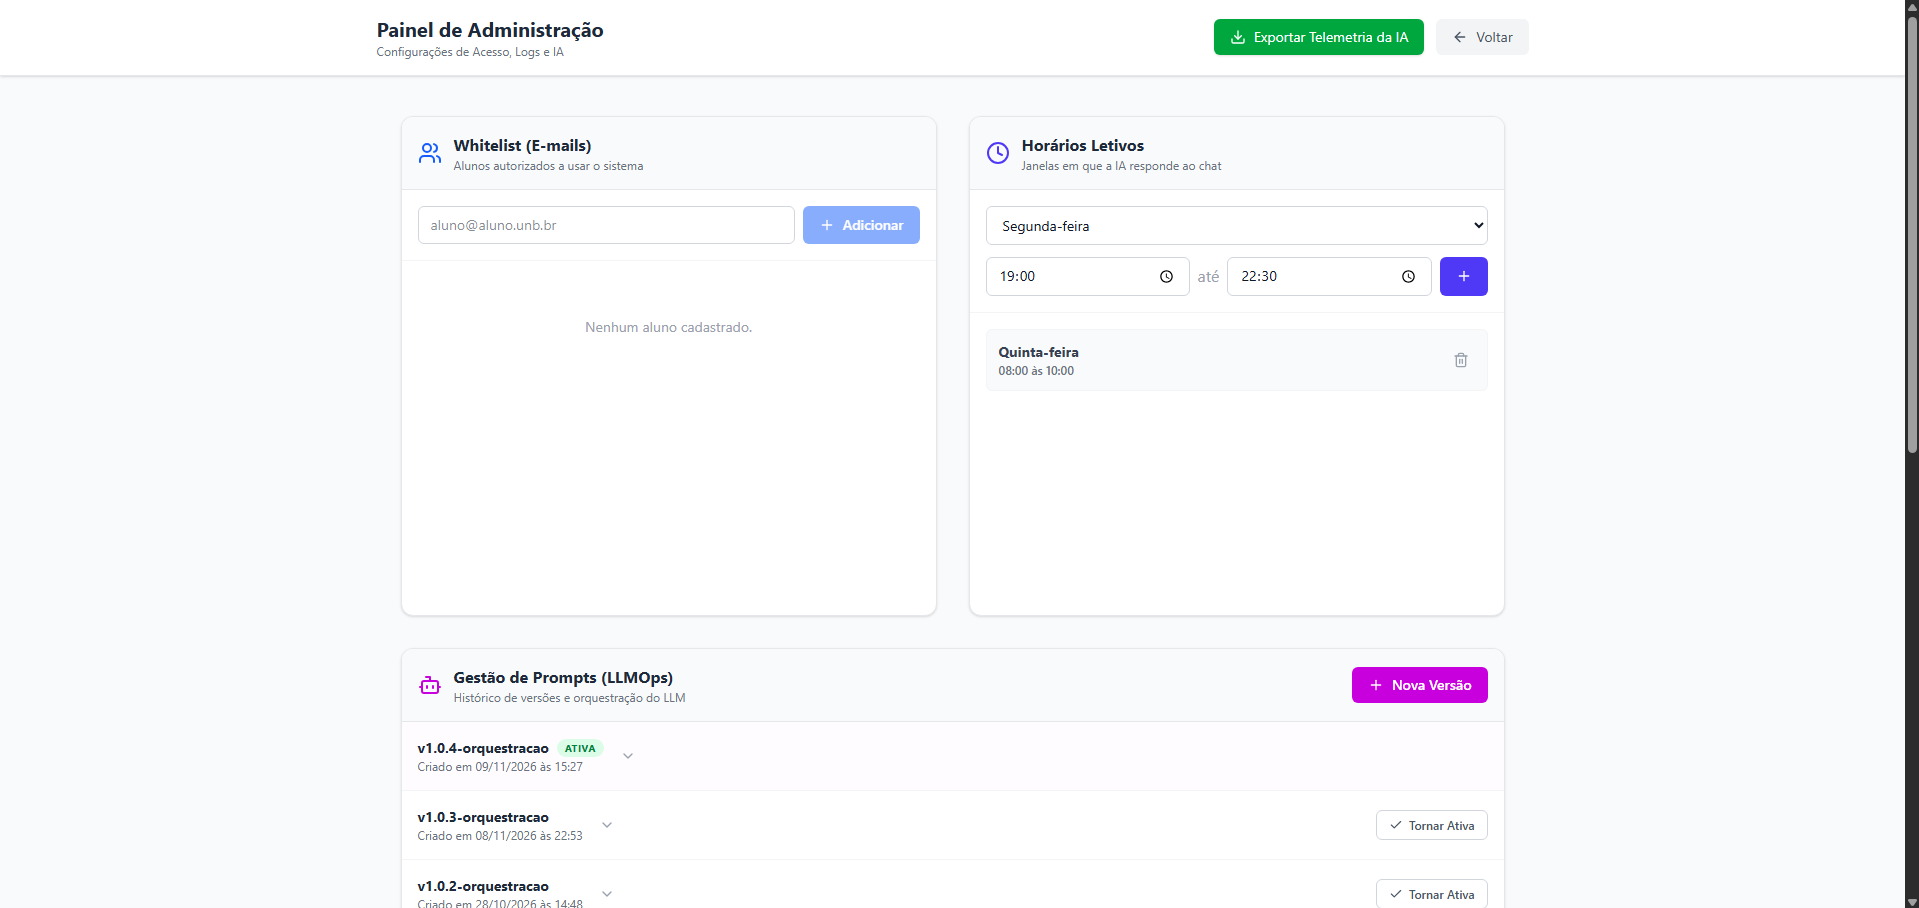
\includegraphics[trim={280px 0px 280px 0px}, clip, width=\textwidth]{figuras/tela_admin1.png}
        \par\smallskip{\footnotesize (a) \textit{Whitelist}, Horários Letivos e Gestão de \textit{Prompts}}
    \end{minipage}
    \hfill
    \begin{minipage}[b]{0.48\textwidth}
        \centering
        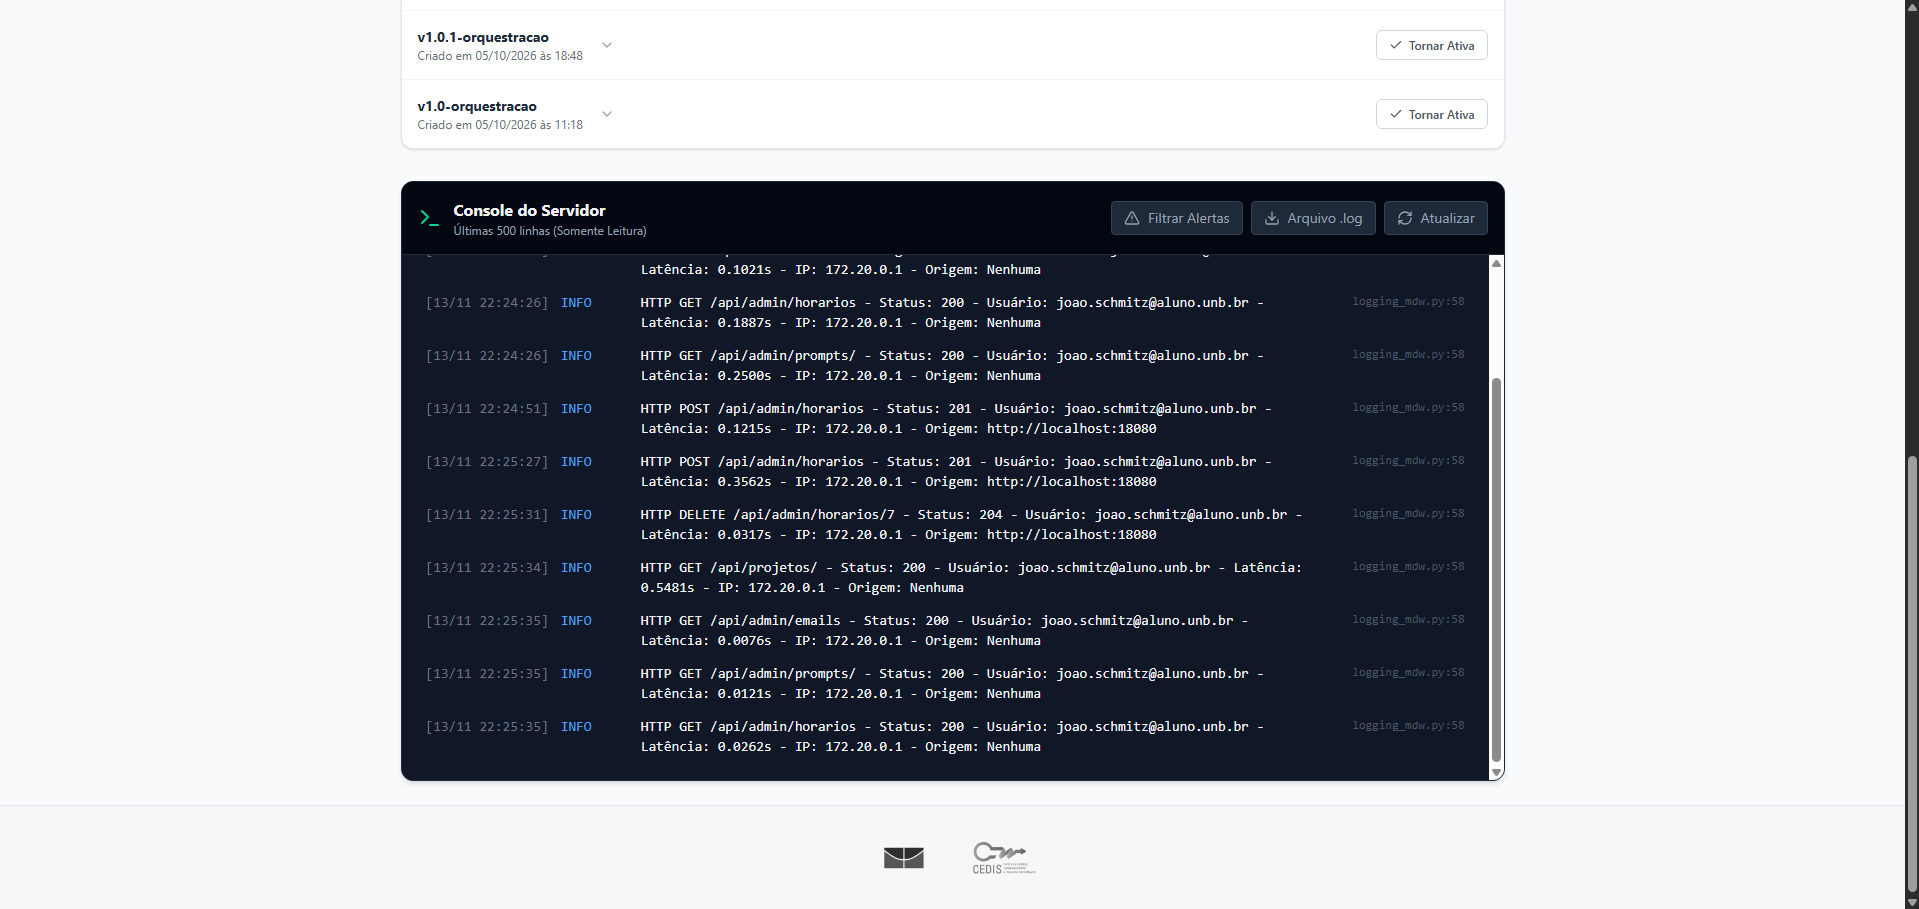
\includegraphics[trim={280px 0px 280px 0px}, clip, width=\textwidth]{figuras/tela_admin2.png}
        \par\smallskip{\footnotesize (b) Console do Servidor e inspeção de \textit{logs}}
    \end{minipage}
    \par\medskip
    \small Fonte: Elaborada pelo autor.
\end{figure}

\subsection{(A3.3) Execução de testes técnicos para validação de estabilidade estrutural}
\label{subsec:exec_a33}

A atividade A3.3 validou a estabilidade estrutural e a escalabilidade da Arquitetura Orientada a Estados (\texttt{v1.0}) por meio de testes automatizados de carga com a ferramenta \textit{Locust}, verificando o suporte a até 50 usuários simultâneos sem esgotamento de conexões no banco de dados. Os testes foram executados na estação de desenvolvimento (processador Intel Core i5-13400F, 16 GB de memória RAM DDR4 e unidade SSD SATA de 256 GB, operando sob ambiente Linux Ubuntu via WSL2 e Docker Engine) comunicando-se via rede externa com a API real da Google Vertex AI. Os contêineres replicaram os parâmetros de produção: PostgreSQL 16 configurado com \texttt{max\_connections = 300}; FastAPI/Uvicorn com 4 processos (\textit{workers}) paralelos (\texttt{pool\_size = 30} e \texttt{max\_overflow = 20} por processo, totalizando capacidade para até 200 conexões simultâneas); e tempo limite (\texttt{timeout}) de leitura no Nginx e no cliente HTTP ajustado para 120 segundos. Utilizou-se um \textit{Token} JWT pré-gerado e desativou-se temporariamente o limite de taxa por usuário para estressar diretamente o núcleo do sistema.

Na \textbf{Bateria 1 (\textit{Step Load Testing})}, a carga foi escalada progressivamente nos patamares de \textbf{5, 10, 20, 35, 50 e 100 usuários virtuais simultâneos} (com duração de 30 segundos por degrau), submetendo mensagens complexas com retorno JSON estruturado (Figura \ref{fig:locust_step_load}). Nos patamares de \textbf{5 a 50 usuários} (alvo pedagógico do projeto), a taxa de falhas manteve-se em \textbf{0\%}, com tempo de resposta estável entre \textbf{3.000 ms e 8.000 ms} e curva do percentil 95 (P95) horizontal, comprovando a eficácia do padrão \textit{Read-Release-Write}. No degrau extremo de \textbf{100 usuários} (vazão aproximada de 10 requisições por segundo), registraram-se recusas decorrentes exclusivamente do limite de taxa contratual (\textit{Rate Limit}) da conta utilizada na Vertex AI, as quais foram interceptadas pelo \textit{backend} com retorno controlado de erro (\texttt{HTTP 503 Service Unavailable}), sem queda do servidor ou corrupção de estado.

\begin{figure}[H]
    \centering
    \caption{Resultados do Teste de Carga em Degraus (\textit{Step Load Test}): Vazão (RPS), Tempo de Resposta (ms) e Usuários Concorrentes}
    \label{fig:locust_step_load}
    
    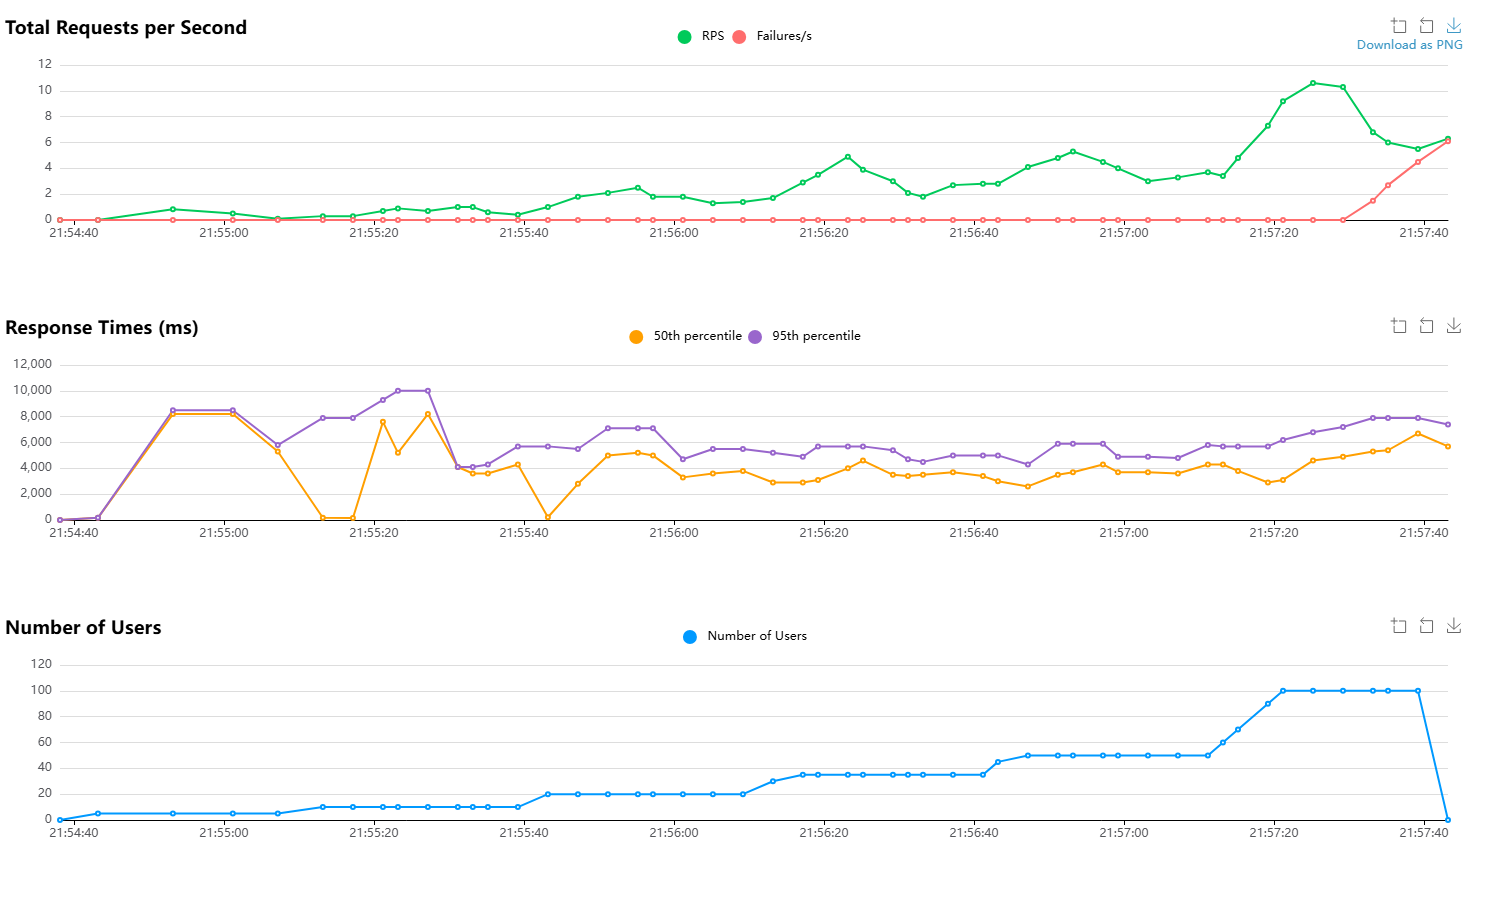
\includegraphics[width=0.92\textwidth]{figuras/locust_step_load.png}
    
    \small Fonte: Elaborada pelo autor via interface do \textit{Locust}.
\end{figure}

Na \textbf{Bateria 2 (\textit{Soak Testing})}, sustentou-se a carga constante de \textbf{50 usuários simultâneos durante 10 minutos ininterruptos} (Figura \ref{fig:locust_soak_test}). Cada usuário virtual operou como uma Máquina de Estados Finita, executando cinco turnos consecutivos de elicitação seguidos do acionamento regressivo da rota ``Desfazer Turno'' (\textit{soft delete} em cascata) até retornar o projeto ao estado inicial. O sistema manteve \textbf{0\% de erros} durante todo o período, alternando entre \textbf{4.000 ms e 18.000 ms} (P95) nas chamadas externas à Vertex AI e latência na \textbf{ordem de poucos milissegundos} nas deleções relacionais em cascata no PostgreSQL. Esse comportamento atestou a ausência de vazamentos de memória (\textit{Memory Leaks}) e confirmou que a criação de índices compostos adicionais (\textbf{T1.07}) não seria necessária para a escala do projeto.

\begin{figure}[H]
    \centering
    \caption{Resultados do Teste de Resistência (\textit{Soak Test}) sob Carga Contínua de 50 Usuários durante 10 Minutos}
    \label{fig:locust_soak_test}
    
    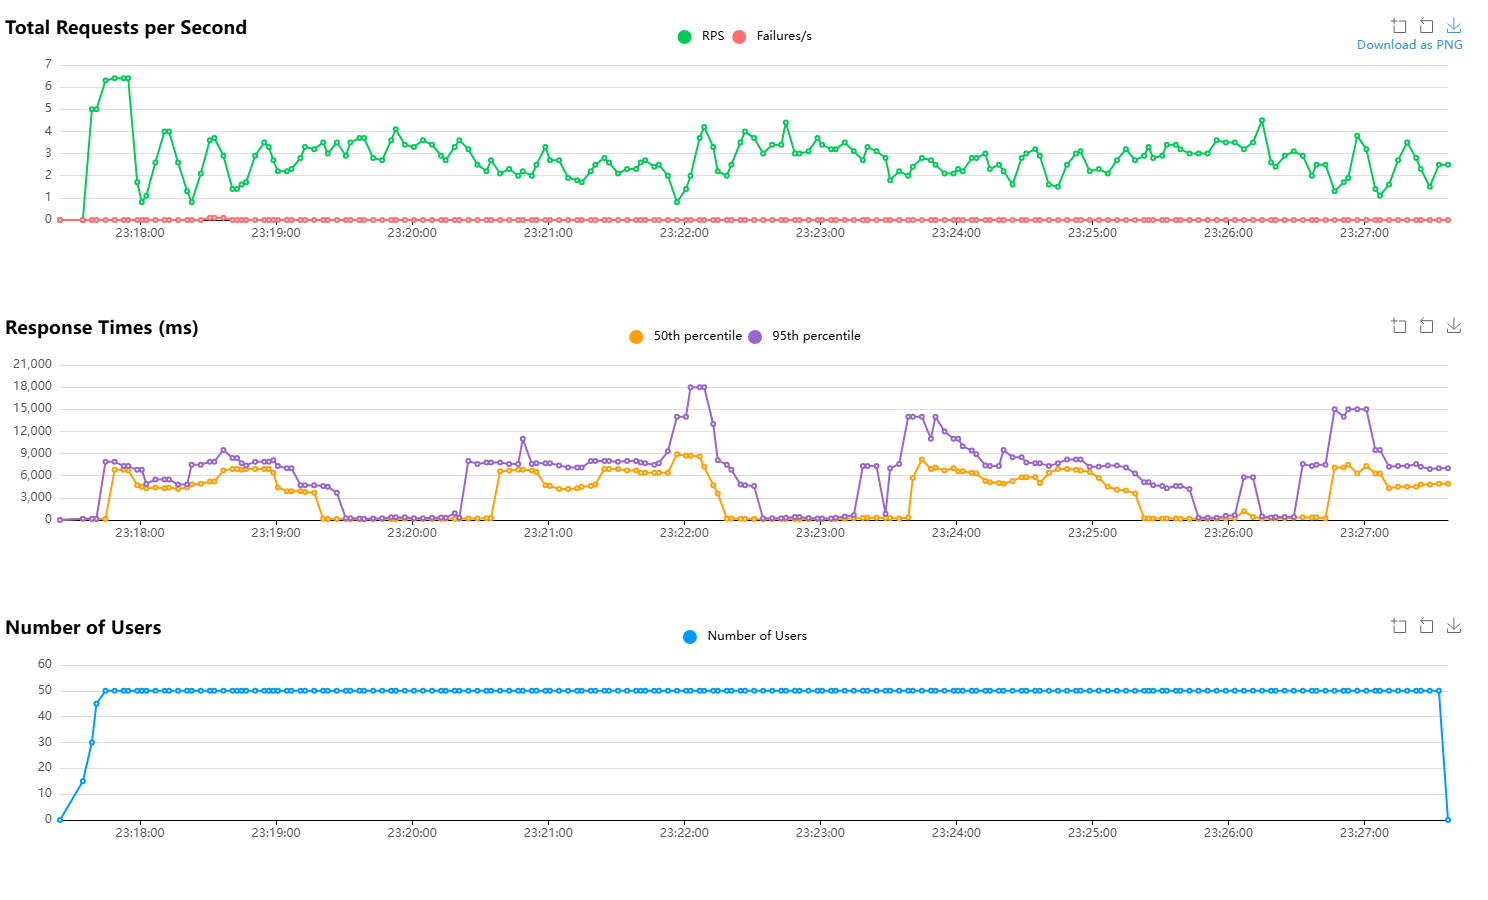
\includegraphics[width=0.92\textwidth]{figuras/locust_soak_test.png}
    
    \small Fonte: Elaborada pelo autor via interface do \textit{Locust}.
\end{figure}

\section{Fase 3: Implantação e Validação em Campo}
\label{sec:execucao_fase3}

Concluídos os testes de estabilidade estrutural na Fase 2, a pesquisa avançou para a validação empírica da Arquitetura Orientada a Estados (\texttt{v1.0}) em ambiente real de ensino, cumprindo as quatro atividades previstas para o quarto objetivo específico do estudo (OE4).

\subsection{(A4.1) Implantação e aplicação do sistema em sala de aula}
\label{subsec:exec_a41}

A atividade A4.1 consistiu na execução presencial do Teste de Aceitação do Usuário (UAT) em duas turmas da disciplina de Requisitos de Software da Universidade de Brasília (UnB, Campus Gama / FCTE). Antes do início das sessões, que ocorreram no dia 22 de outubro de 2026, os e-mails institucionais (\texttt{@aluno.unb.br}) dos líderes de cada equipe foram previamente cadastrados na \textit{Whitelist} da plataforma (\textbf{US1.06}), e as janelas de horário letivo correspondentes aos turnos das aulas foram ativadas no Painel de Administração (\textbf{US1.09}). A distribuição dos estudantes nas duas sessões ocorreu da seguinte forma:

\begin{itemize}
    \item \textbf{Turma 1 (das 08h00 às 09h50):} Dos 44 estudantes matriculados, 38 estiveram presentes em laboratório (86,4\% de presença), organizados em 7 equipes de projeto.
    \item \textbf{Turma 2 (das 10h00 às 11h50):} Dos 45 estudantes matriculados, 40 estiveram presentes em laboratório (88,9\% de presença), organizados em 7 equipes de projeto.
\end{itemize}

No total, a validação em campo contou com a participação presencial de \textbf{78 estudantes distribuídos em 14 equipes ativas} simultaneamente. Conforme o protocolo metodológico estabelecido na Seção \ref{sec:fase3}, cada equipe utilizou como base o escopo real de seu projeto semestral da disciplina, cujo levantamento tradicional de requisitos já havia sido elaborado previamente pelo grupo. Durante a sessão, os estudantes interagiram com o ElicitBot em regime de revezamento de operador a cada fase da Máquina de Estados, enquanto os demais integrantes discutiam coletivamente as perguntas do assistente e inspecionavam os artefatos gerados na barra lateral.

\subsection{(A4.2) Coleta de métricas de uso e aplicação do questionário de avaliação}
\label{subsec:exec_a42}

Durante as duas sessões presenciais, o comportamento operacional do servidor foi acompanhado em tempo real por meio do Console do Servidor no Painel de Administração (\textbf{US3.05}). Paralelamente, o sistema persistiu no PostgreSQL o histórico completo de mensagens, o estado de progressão das equipes nos 14 projetos instanciados, os artefatos extraídos nas oito categorias de domínio e os registros de telemetria de cada chamada à API na entidade \texttt{MetricaLLM}, posteriormente exportados em formato CSV (\textbf{US3.04}).

Ao término da atividade prática em laboratório, foi disponibilizado o Questionário de Avaliação Estruturado para preenchimento individual e assíncrono pelos estudantes que participaram da dinâmica. O instrumento foi composto por 32 variáveis distribuídas em três partes: uma questão fechada de controle de funil para identificar a etapa máxima da Máquina de Estados alcançada pela equipe durante a aula; 20 afirmações avaliativas em escala Likert de 5 pontos (\texttt{1 = Discordo Totalmente} a \texttt{5 = Concordo Totalmente}); e 10 questões abertas opcionais voltadas ao relato de incongruências semânticas, falhas de interface ou estado e sugestões de evolução.

Dos 78 estudantes presentes nas duas turmas, foram obtidas \textbf{$N = 65$ respostas individuais válidas}, correspondendo a uma taxa de retorno amostral de \textbf{83,3\%}. Para assegurar a privacidade dos participantes e permitir a rastreabilidade cruzada na pesquisa, os respondentes foram anonimizados sob os identificadores sequenciais \texttt{[P1]} a \texttt{[P65]}. A base de dados e o instrumento completo aplicado encontram-se disponíveis no repositório oficial do projeto\footnote{Instrumento de coleta e planilha de respostas disponíveis em: \url{https://github.com/CedisUnB/ElicitBot-v2/tree/main/docs/evaluation}.}.

\subsection{(A4.3) Análise qualitativa dos relatos e sistematização do plano de ação}
\label{subsec:exec_a43}

Na atividade A4.3, as respostas submetidas nos 10 campos abertos do formulário pelos 65 estudantes participantes foram processadas por meio de Triagem Técnica de Incidentes e Categorização Indutiva de Relatos. Os apontamentos foram consolidados em 18 tópicos temáticos e classificados em três categorias de encaminhamento. O mapeamento integral dessa análise, contendo a descrição detalhada, a frequência de ocorrência ($f$), a rastreabilidade aos identificadores dos respondentes (\texttt{[P1]} a \texttt{[P65]}) e o respectivo plano de ação ou justificativa técnica, encontra-se documentado no Apêndice \ref{apendice:triagem_qualitativa}.

\begin{itemize}
    \item \textbf{Categoria 1 (Correções Imediatas, \texttt{CI-01} a \texttt{CI-04}):} Reúne os gargalos de usabilidade na interface atual e as falhas sistêmicas ou de sincronização de estado com impacto direto na integridade do projeto elicitado. Foram mapeados quatro pontos prioritários: as limitações de usabilidade no componente de entrada de dados, como ausência de redimensionamento vertical, perda de foco do cursor e falta de atalho para quebra de linha (\texttt{CI-01}, com 22 relatos); a falha de concorrência na Fase 11 (\texttt{Validação de Requisitos}), quando o agente tentava atualizar um requisito e submetê-lo à validação no mesmo turno ou alterar simultaneamente o atributo de pendências junto a outros dados do artefato, além da falta de mensagens de erro claras (\texttt{CI-02}, com 14 relatos); as fricções de navegação por ausência de rolagem automática no \textit{chat} e fechamento de modais restrito ao botão ``X'' (\texttt{CI-03}, com 5 relatos); e os casos pontuais de duplicação semântica na geração de artefatos ou menção no diálogo a \textit{Tags} já excluídas (\texttt{CI-04}, com 5 relatos).
    \item \textbf{Categoria 2 (Limitações Aceitáveis e Delimitação de Escopo, \texttt{LA-01} a \texttt{LA-07}):} Agrupa comportamentos derivados de decisões metodológicas da pesquisa, que não devem ser removidos para não invalidar a engenharia de \textit{prompt} proposta, além de variações inerentes à natureza probabilística de LLMs já mitigadas pela arquitetura \textit{Human-in-the-Loop}. Esta categoria abrangeu sete aspectos: o uso da edição manual na barra lateral para refinar artefatos ou ajustar títulos genéricos definidos na criação do projeto (\texttt{LA-01}, com 12 relatos); a concisão dos artefatos e da granularidade do MVP para evitar extrapolações não fornecidas pelo aluno (\texttt{LA-02}, com 7 relatos); as variações não determinísticas pontuais de atenção e o rigor nas confirmações de transição de fase frente a respostas vagas (\texttt{LA-03}, com 6 relatos); a resiliência a desvios de domínio, respondendo brevemente a provocações externas e reconduzindo o diálogo à etapa exata da elicitação sem esforço extra com \textit{guardrails} (\texttt{LA-04}, com 4 relatos); a blindagem metodológica no formato Connextra de Histórias de Usuário frente a tentativas de uso de outros \textit{frameworks} como FDD (\texttt{LA-05}, com 3 relatos); a condução e validação unitária de requisitos em vez de processamento em lote (\texttt{LA-06}, com 3 relatos); e o tratamento do estudante como cliente ou \textit{stakeholder} na simulação de entrevista (\texttt{LA-07}, com 2 relatos).
    \item \textbf{Categoria 3 (Trabalhos Futuros, \texttt{TF-01} a \texttt{TF-07}):} Sistematiza as sugestões discentes de inovação funcional, novos módulos de experiência do usuário e adição de tecnologias que extrapolam o escopo atual. Os pontos levantados compreenderam: a ingestão de arquivos (PDF, Markdown, \textit{links}) e contexto multimodal com imagens no \textit{chat} (\texttt{TF-01}, com 10 relatos); a interface de voz via transcrição de áudio por microfone (\texttt{TF-02}, com 4 relatos); uma camada de \textit{onboarding} visual com dicas conceituais sobre etapas e artefatos (\texttt{TF-03}, com 3 relatos); o suporte parametrizável a múltiplos \textit{frameworks} de Engenharia de Requisitos (\texttt{TF-04}, com 3 relatos); a visualização em grafo da matriz de rastreabilidade e geração de diagramas (\texttt{TF-05}, com 2 relatos); a transparência de raciocínio via componente expansível de \textit{Modo Pensamento} (\texttt{TF-06}, com 1 relato); e um botão de interrupção imediata da geração em andamento (\textit{Stop Generation}) (\texttt{TF-07}, com 1 relato).
\end{itemize}

\subsection{(A4.4) Aplicação das correções imediatas para refinamento do sistema}
\label{subsec:exec_a44}

Encerrando a Fase 3 e o Ciclo de Design da DSR, a atividade A4.4 executou a manutenção corretiva e evolutiva do software, implementando no repositório do projeto as quatro intervenções mapeadas na Categoria 1 do plano de ação (\texttt{CI-01} a \texttt{CI-04}):

\begin{enumerate}
    \item \textbf{Reformulação do Componente de Entrada de Dados (\texttt{CI-01}):} O campo de formulário padrão de linha única no \textit{frontend} (React) foi substituído por uma caixa de texto dinâmica autoexpansível com suporte a múltiplas linhas, preservação de foco do cursor e remapeamento de eventos de teclado (envio via \texttt{Enter} e quebra de linha via \texttt{Shift + Enter}), facilitando a redação e revisão de respostas extensas.
    \item \textbf{Resolução da Concorrência na Validação de Requisitos e Tratamento de Erros (\texttt{CI-02}):} O \textit{System Prompt} e a orquestração do Motor de Operações no \textit{backend} foram modificados para remover a exclusividade na alteração do atributo \texttt{pendencias\_validacao} durante edições e exigir que a operação de atualização (\texttt{atualizar}) seja persistida e auditada deterministicamente pelo \textit{backend} antes da emissão do comando final de aprovação (\texttt{validar}), ignorando com segurança acionamentos prematuros no mesmo turno. Adicionalmente, o tratamento de mensagens de erro na interface foi aprimorado para apresentar retornos claros ao usuário.
    \item \textbf{Melhorias de Navegação no \textit{Chat} e Fechamento de Modais (\texttt{CI-03}):} Foram implementadas âncoras de rolagem automática (\textit{auto-scroll}) no contêiner de mensagens a cada turno enviado ou recebido, bem como ouvintes de evento para permitir o fechamento de modais de artefatos diretamente pelo clique na camada de fundo (\textit{backdrop}).
    \item \textbf{Refinamento das Diretrizes de Manutenção de Identidade e Exclusão no \textit{Prompt} (\texttt{CI-04}):} O \textit{System Prompt} foi atualizado na seção de \textit{``Manutenção de Identidade por Tag e Controle de Duplicatas''}, restringindo a emissão de comandos \texttt{criar} quando houver equivalência semântica com elementos já existentes na memória e garantindo que \textit{Tags} de artefatos descartados sejam tratadas como inexistentes pelo modelo.
\end{enumerate}

\section{Fase 4: Avaliação e Análise de Resultados}
\label{sec:execucao_fase4}

Concluída a validação presencial em laboratório e a aplicação das correções imediatas na Fase 3, a Fase 4 concentrou-se no processamento dos dados coletados para responder ao quinto objetivo específico da pesquisa (OE5). A presente seção expõe de forma direta os dados quantitativos apurados na atividade A5.1, enquanto a interpretação crítica desses indicadores, a triangulação metodológica com os relatos qualitativos (A5.2) e a análise comparativa entre as versões da ferramenta (A5.3) são desenvolvidas no Capítulo \ref{cap:analise}.

\subsection{(A5.1) Consolidação, higienização e apuração estatística dos dados quantitativos}
\label{subsec:exec_a51}

A apuração quantitativa processou as respostas fechadas em escala ordinal (Likert de 1 a 5 pontos) e a métrica categórica de progressão no fluxo de elicitação obtidas junto aos $N = 65$ estudantes respondentes. Os 20 itens avaliativos do instrumento foram agrupados em cinco dimensões teóricas (construtos) alinhadas às fases da Máquina de Estados do ElicitBot:

\begin{itemize}
    \item \textbf{Condução Conversacional e Controle de Processo (D1, 6 itens):} Avalia o respeito à sequência lógica de fases, a cadência de perguntas por turno, a investigação do problema real antes da solução, a retenção de contexto, a solicitação de confirmação nas transições e a adequação da linguagem.
    \item \textbf{Modelagem do Problema e Domínio de Negócio (D2, 5 itens):} Avalia a compreensão da dor real, o levantamento das partes interessadas (\textit{stakeholders}), o mapeamento de interesses e necessidades, o foco em valor e objetivos de negócio mensuráveis e o isolamento semântico de restrições.
    \item \textbf{Concepção e Viabilidade de Soluções (D3, 3 itens):} Avalia o alinhamento das alternativas propostas aos problemas e objetivos, a adesão às restrições técnicas e orçamentárias e a clareza e viabilidade prática das soluções.
    \item \textbf{Especificação, Verificabilidade e Rastreabilidade de Requisitos (D4, 4 itens):} Avalia a adesão ao formato padrão Connextra de Histórias de Usuário, a fidelidade das regras de negócio extraídas, a verificabilidade dos critérios de aceitação e a manutenção de vínculos de rastreabilidade.
    \item \textbf{Satisfação Geral e Potencial de Adoção (D5, 2 itens):} Avalia a satisfação global com a interação e os resultados obtidos, bem como o potencial de adoção da ferramenta em projetos acadêmicos ou profissionais futuros.
\end{itemize}

\subsubsection*{Consistência Interna e Funil de Progressão na Elicitação}

Inicialmente, foi verificada a confiabilidade do instrumento por meio do coeficiente Alfa de Cronbach ($\alpha$), considerando os registros com preenchimento integral em todas as 20 variáveis ($n = 52$). O questionário obteve \textbf{$\alpha = 0,877$}, índice superior ao limiar de referência adotado na literatura ($\alpha \ge 0,70$), confirmando a consistência interna das respostas.

Em seguida, foi tabulada a variável categórica \textit{Progresso na Elicitação}, que registrou a etapa máxima da Máquina de Estados alcançada por cada participante durante o tempo da sessão prática. A distribuição de retenção ao longo do fluxo é apresentada na Tabela \ref{tab:funil_progressao}.

\noindent
{
\footnotesize 
\renewcommand{\arraystretch}{1.15}
\setlength{\LTleft}{0pt}
\setlength{\LTright}{0pt}

\begin{xltabular}{\textwidth}{|>{\raggedright\arraybackslash}X|c|c|c|>{\raggedright\arraybackslash}p{3.0cm}|}
    \caption{Funil de Progressão e Retenção de Participantes na Máquina de Estados ($N = 65$)}
    \label{tab:funil_progressao} \\
    \toprule
    \textbf{Etapa Máxima Atingida no Fluxo} & \textbf{Freq. Absoluta ($n$)} & \textbf{Freq. Relativa (\%)} & \textbf{Freq. Acumulada ($\ge$ Etapa)} & \textbf{Identificadores (Paradas Prematuras)} \\
    \midrule
    \endfirsthead

    \bottomrule
    \multicolumn{5}{c}{\small Fonte: Elaborada pelo autor a partir dos dados da validação ($N = 65$).} \\
    \endlastfoot
    
    Confirmar Escopo (Fase 12, Final) & 27 & 41,5\% & 41,5\% & N/A \\
    \midrule
    Validação de Requisitos (Fase 11, Penúltima) & 8 & 12,3\% & 53,8\% & N/A \\
    \midrule
    Requisitos Funcionais (Fase 10, Antepenúltima) & 25 & 38,5\% & \textbf{92,3\%} & N/A \\
    \midrule
    Validação de Solução (Fase 9) & 2 & 3,1\% & 95,4\% & \texttt{[P3, P55]} \\
    \midrule
    Objetivos de Negócio (Fase 5) & 2 & 3,1\% & 98,5\% & \texttt{[P33, P49]} \\
    \midrule
    Contexto (Fase 1, Inicial) & 1 & 1,5\% & 100,0\% & \texttt{[P44]} \\
    \midrule
    \textbf{Total de Participantes Avaliados} & \textbf{65} & \textbf{100,0\%} & N/A & N/A \\
\end{xltabular}
}

Os dados da Tabela \ref{tab:funil_progressao} demonstram que \textbf{92,3\% dos participantes} ($n = 60$ de 65) concluíram todas as etapas de entendimento de domínio e concepção de solução, atingindo ao menos a Fase 10 (\texttt{Requisitos Funcionais}), sendo que 41,5\% ($n = 27$) finalizaram integralmente a Fase 12 (\texttt{Confirmar Escopo}) e 50,8\% ($n = 33$) encerraram o horário de laboratório concentrados nas Fases 10 e 11. Apenas 5 participantes (7,7\%, correspondentes aos respondentes \texttt{[P3, P33, P44, P49, P55]}) relataram interrupção em fases preliminares ou intermediárias.

\subsubsection*{Estatísticas Descritivas por Critério e Dimensão e Higienização Condicional}

Para cada um dos 20 critérios e 5 dimensões, foram calculados o número de respostas válidas ($N$), a Média ($\mu$), o Desvio Padrão ($\sigma$), a Mediana ($Md$), a Moda ($Mo$), a Taxa de Aprovação Positiva (\textit{Top-2 Box}, proporção de notas 4 e 5), o percentual de nota máxima ($= 5$) e a distribuição absoluta de frequências nos cinco níveis da escala (\texttt{[1, 2, 3, 4, 5]}). A média global do instrumento, considerando todos os 20 critérios, foi de \textbf{$\mu = 4,49$}, sendo que \textbf{todos os 20 itens apresentaram Mediana ($Md = 5,0$) e Moda ($Mo = 5,0$) iguais à nota máxima da escala}. A Tabela \ref{tab:estatisticas_descritivas} consolida os resultados ordenados pela média dentro de cada dimensão.

\noindent
{
\footnotesize 
\renewcommand{\arraystretch}{1.15}
\setlength{\LTleft}{0pt}
\setlength{\LTright}{0pt}

\begin{xltabular}{\textwidth}{|>{\raggedright\arraybackslash}p{2.3cm}|>{\raggedright\arraybackslash}X|c|c|c|c|c|c|}
    \caption{Estatísticas Descritivas e Distribuição de Respostas por Dimensão e Critério ($Md = 5,0$ e $Mo = 5,0$ em todos os itens)}
    \label{tab:estatisticas_descritivas} \\
    \toprule
    \textbf{Dimensão} & \textbf{Critério Avaliado} & \textbf{$N$} & \textbf{Média ($\mu$)} & \textbf{Desvio ($\sigma$)} & \textbf{\textit{Top-2 Box}} & \textbf{Nota Máx. ($=5$)} & \textbf{Dist. \texttt{[1,2,3,4,5]}} \\
    \midrule
    \endfirsthead

    \multicolumn{8}{c}%
    {{\bfseries \tablename\ \thetable{} -- continuação da página anterior}} \\
    \toprule
    \textbf{Dimensão} & \textbf{Critério Avaliado} & \textbf{$N$} & \textbf{Média ($\mu$)} & \textbf{Desvio ($\sigma$)} & \textbf{\textit{Top-2 Box}} & \textbf{Nota Máx. ($=5$)} & \textbf{Dist. \texttt{[1,2,3,4,5]}} \\
    \midrule
    \endhead

    \midrule \multicolumn{8}{r}{{Continua na próxima página...}} \\
    \endfoot

    \bottomrule
    \multicolumn{8}{c}{\small Fonte: Elaborada pelo autor a partir dos dados quantitativos da validação ($N = 65$).} \\
    \endlastfoot
    
    \textbf{D1: Condução} \newline ($\mu = 4,58$) & Validação de Transição & 65 & 4,83 & 0,52 & 96,9\% & 87,7\% & \texttt{[0, 1, 1, 6, 57]} \\
    \cline{2-8}
    & Adesão ao Fluxo Lógico & 65 & 4,78 & 0,41 & 100,0\% & 78,5\% & \texttt{[0, 0, 0, 14, 51]} \\
    \cline{2-8}
    & Investigação do Problema Real & 65 & 4,68 & 0,59 & 93,8\% & 73,8\% & \texttt{[0, 0, 4, 13, 48]} \\
    \cline{2-8}
    & Adequação da Linguagem & 65 & 4,60 & 0,55 & 96,9\% & 63,1\% & \texttt{[0, 0, 2, 22, 41]} \\
    \cline{2-8}
    & Cadência de Perguntas & 65 & 4,48 & 0,71 & 87,7\% & 60,0\% & \texttt{[0, 0, 8, 18, 39]} \\
    \cline{2-8}
    & Retenção de Contexto & 65 & 4,09 & 1,17 & 69,2\% & 53,8\% & \texttt{[3, 3, 14, 10, 35]} \\
    \midrule
    \textbf{D2: Negócio} \newline ($\mu = 4,42$) & Compreensão da Dor Real & 64 & 4,52 & 0,62 & 93,8\% & 57,8\% & \texttt{[0, 0, 4, 23, 37]} \\
    \cline{2-8}
    & Levantamento dos Envolvidos & 64 & 4,52 & 0,71 & 90,6\% & 62,5\% & \texttt{[0, 1, 5, 18, 40]} \\
    \cline{2-8}
    & Isolamento Semântico de Restrições & 64 & 4,39 & 0,83 & 84,4\% & 57,8\% & \texttt{[0, 2, 8, 17, 37]} \\
    \cline{2-8}
    & Foco em Valor e Resultados & 64 & 4,36 & 0,82 & 84,4\% & 54,7\% & \texttt{[0, 2, 8, 19, 35]} \\
    \cline{2-8}
    & Interesses dos Envolvidos & 63 & 4,33 & 0,84 & 87,3\% & 50,8\% & \texttt{[1, 1, 6, 23, 32]} \\
    \midrule
    \textbf{D3: Soluções} \newline ($\mu = 4,50$) & Adesão às Restrições & 63 & 4,63 & 0,55 & 96,8\% & 66,7\% & \texttt{[0, 0, 2, 19, 42]} \\
    \cline{2-8}
    & Alinhamento da Solução & 64 & 4,53 & 0,64 & 95,3\% & 59,4\% & \texttt{[0, 1, 2, 23, 38]} \\
    \cline{2-8}
    & Clareza e Viabilidade das Soluções & 62 & 4,32 & 0,83 & 83,9\% & 51,6\% & \texttt{[0, 2, 8, 20, 32]} \\
    \midrule
    \textbf{D4: Requisitos} \newline ($\mu = 4,50$) & Rastreabilidade de Requisitos & 58 & 4,60 & 0,56 & 96,6\% & 63,8\% & \texttt{[0, 0, 2, 19, 37]} \\
    \cline{2-8}
    & Adesão ao Formato Padrão & 61 & 4,57 & 0,88 & 90,2\% & 73,8\% & \texttt{[2, 0, 4, 10, 45]} \\
    \cline{2-8}
    & Fidelidade de Regras & 55 & 4,42 & 0,69 & 89,1\% & 52,7\% & \texttt{[0, 0, 6, 20, 29]} \\
    \cline{2-8}
    & Verificabilidade & 57 & 4,40 & 0,70 & 87,7\% & 52,6\% & \texttt{[0, 0, 7, 20, 30]} \\
    \midrule
    \textbf{D5: Geral} \newline ($\mu = 4,39$) & Interação e Resultados & 65 & 4,40 & 0,70 & 90,8\% & 50,8\% & \texttt{[0, 1, 5, 26, 33]} \\
    \cline{2-8}
    & Potencial de Uso & 65 & 4,38 & 0,84 & 83,1\% & 58,5\% & \texttt{[0, 2, 9, 16, 38]} \\
\end{xltabular}
}

Por fim, foi executado o procedimento de \textbf{Higienização Condicional}. Observou-se na Tabela \ref{tab:estatisticas_descritivas} que o total de respostas válidas ($N$) reduz-se de $N = 65$ nas dimensões iniciais para $N = 55$ a $61$ na dimensão de Requisitos (D4), refletindo abstenções voluntárias de participantes que não concluíram as etapas finais. Contudo, parte dos 5 respondentes que encerraram a sessão antes da Fase 10 (\texttt{[P3, P33, P44, P49, P55]}) preencheu avaliações para itens de D3 e/ou D4. Ao aplicar a filtragem estrita por fase atingida, recalculando os indicadores de D3 e D4 exclusivamente para o subgrupo de 60 participantes que efetivamente alcançou a etapa de Requisitos Funcionais, verificou-se variação máxima de \textbf{$\pm 0,02$ ponto} nas médias de D4 (\textit{Adesão ao Formato Padrão} passou de $\mu = 4,57$ para $\mu = 4,55$; \textit{Fidelidade de Regras}, de $\mu = 4,42$ para $\mu = 4,40$; \textit{Verificabilidade}, de $\mu = 4,40$ para $\mu = 4,41$; e \textit{Rastreabilidade de Requisitos} permaneceu inalterada em $\mu = 4,60$), mantendo-se $Md = 5,0$ em todos os critérios.

Com a exposição direta dos resultados de execução e dos levantamentos empíricos concluída, o capítulo a seguir aprofunda a análise crítica desses dados, a triangulação metodológica entre achados quantitativos e qualitativos (A5.2), a comparação sistemática com a versão original da ferramenta (A5.3), as contribuições científicas e práticas e as limitações do estudo.